\documentclass[12pt]{extarticle}
\usepackage[utf8]{inputenc}
\usepackage{amsmath}
\usepackage{hyperref}
\usepackage{float}
\usepackage{graphicx}
\usepackage{caption}
\usepackage[export]{adjustbox}
\usepackage{amssymb}
\usepackage{hyperref}
\usepackage{algorithm2e}
\usepackage{multirow}

\RestyleAlgo{ruled}

\newtheorem{theorem}{Theorem}[section]
\newtheorem{corollary}{Corollary}[theorem]
\newtheorem{lemma}[theorem]{Lemma}

\newcommand{\quotes}[1]{``#1''}

\title{CM project - 32 NonML}
\author{Luca Moroni (635966), Diego Arcelli (647979)}
\date{Febbraio 2022}

\linespread{1.2}
\usepackage[a4paper,margin=1in,footskip=0.25in]{geometry}


\begin{document}

\maketitle

\section{Introduzione}
In questa sezione andremo a definire il problema soggetto del presente elaborato. Il problema da noi selezionato è il numero 32 della sezione   \quotes{progetti nonML}.
\subsection{Il problema}
Il problema consiste nel trovare il minimo di una funzione quadratica, il cui dominio è vincolato, il problema nello specifico rientra nella tipologia \quotes{knapsack quadratic non-separable problems}.\\
\[\min_x \{x'Qx + q'x : a'x \geq b, l \leq x \leq u\}\]
Dove $x \in \mathbb{R}^n$ mentre $q, a, l, u$  sono vettori fissati in $\mathbb{R}^n$ con $0 \leq l < u$, e $Q \in \mathbb{R}^{n \times n}$ è una matrice semi-definita positiva.\\
La funzione obiettivo, a seconda della scelta di $Q$ e $q$, puo essere limitata inferiormente oppure no, nel caso di matrice con autovalori non strettamente positivi è possibile avere funzioni non limitate inferiormente. Avendo un problema vincolato la nostra funzione ammetterà un unico valore di minimo nella regione ammissibile se non vuota, rientrando nelle ipotesi del teorema del valore estremo di Weirestrass, ovvero, la nostra funzione obiettivo è continua ed la nostra regione ammissibile, se non vuota, è chiusa e limitata ovvero un insieme compatto. Non è garantita invece l'unicità del punto di minimo.
\section{Algoritmo risolutivo}
Per la risoluzione di tale problema la traccia ci ha esplicitamente richiesto di utilizzare un metodo iterativo di discesa del gradiente, applicando però la tecnica della gradient projection in quanto ci troviamo a dover minimizzare una funzione vincolata. Si è deciso di applicare la metodologia di Wolfe la quale consiste, informalmente, nel calcolare il gradiente in un punto, muoversi nella direzione opposta utilizzando un qualche metodo di scelta del passo, e poi proiettare il punto trovato all'interno della regione ammissibile.\\
Si presentano ora due problematiche, capire come proiettare il punto trovato ad ogni iterazione all'interno della regione ammissibile e capire quando fermarsi.
Quest'ultima problematica viene risolta basandosi sul fatto che in un problema di ottimizzazione vincolato un punto stazionario è un punto $x$ tale che $x = projection(x + \alpha\nabla f(x))$ $\forall \alpha \geq 0$.\\
Definiamo dunque come stopping criteria la condizione che la norma della differenza tra la proiezione del punto successivo e il punto attuale sia minore di un certo valore soglia $\epsilon$. Al netto di un passo sufficientemente grande (tratteremo questo aspetto in una sottosezione successiva) abbiamo due casi. Nel caso in cui il punto successivo sia interno alla regione ammissibile, allora questo stopping criteria si attiverà quando il gradiente è vicino a 0 e data la convessita della funzione obiettivo è condizione necessaria e sufficiente per l'ottimalità del punto. Nel caso in cui lo spostamento ci porta fuori dalla regione ammissibile, se la proiezione ci porterà sul bordo molto vicino al punto del passo precedente allora la direzione di spostamento, ovvero l'antigradiente, approssimativamente (per $\epsilon$ abbastanza piccolo) apparterrà al cono duale, generato dai vincoli che rappresentano il bordo della regione ammissibile, quindi per il lemma di Farkas ogni direzione $d$ appartenente all'insieme delle direzioni ammissibili è una direzione di crescita in quanto $\nabla f(x)'d \geq 0$, perciò il punto è un punto di minimo locale nella regione ammissibile. Si faccia riferimento a \cite{pgm_method} per una riscontro formale.\\
Per quanto riguarda invece la tecnica di proiezione la descriveremo nella seguente sottosezione.
\SetKwComment{Comment}{/* }{ */}
\begin{algorithm}
\caption{Gradient Projection Algorithm}
\KwData{$\{f (function), a, u, l, b\}, x_0, \epsilon, \epsilon'$}
\While{$\| x_i - x_{i-1} \| \leq \epsilon$}{
  $d \gets -\nabla f(x_i)$\\
  $\alpha \gets get\_step\_size()$\\
  $y \gets x_i + \alpha d$\\
  $x_i \gets project(\{f (function), a, u, l, b\}, y, \epsilon')$\\
}
\end{algorithm}
\subsection{Metodo di proiezione}
Una volta calcolato il punto derivante dal passo di discesa del gradiente si verifica l'appartenenza alla regione ammissibile, nel qual caso la proiezione non avrà alcun effetto, nel caso, invece in cui il punto esca fuori dalla regione ammissibile, definiamo la proiezione come il punto appartenente alla regione ammissibile che minimizza la distanza euclidea dal punto calcolato. Dall'impostazione appena esplicitata ci rendiamo conto che il problema della proiezione è un problema analogo a quello di partenza ma piu semplice, definiamolo formalmente.
\[\min_{x} \{\|x - \hat{x} \|_2^2 : a'x \geq b, l \leq x \leq u \}\]
Dove $a, b, l, u$ sono definite come nella formulazione del problema originale, ed $\hat{x}$ è il vettore rappresentante il punto derivante dal passo di discesa del gradiente.\\
Riscriviamo la funzione obiettivo del problema di proiezione.
\[\min_x \{(x - \hat{x})'I(x - \hat{x}) : a'x \geq b, l \leq x \leq u \}\]
Dove $I$ è la matrice identità. Il problema di Proiezione è definito come \texttt{Knapsack Separable Quadratic Problem}, per questa specifica tipologia esistono metodi risolutivi che non richiedono la discesa del gradiente. Prima di addentrarci nella descrizione del metodo riformuliamo il problema.\\
Definiamo $\widetilde{x} = x - \hat{x}$ e perciò $x = \widetilde{x} + \hat{x}$ sostituendo abbiamo che, $\widetilde{x} \geq l - \hat{x}$, $\widetilde{x} \leq u - \hat{x}$ definiamo perciò $\widetilde{l} = l - \hat{x}$ e $\widetilde{u} = u - \hat{x}$, inoltre il vincolo $a'x \geq b$ diventa $a'\widetilde{x} \geq b - a'\hat{x}$ volendo inoltre essere consistenti con la formulazione del problema in [2] dobbiamo trasformare tale vincolo nel seguente $-a'\widetilde{x} \leq -(b - a'\hat{x})$ e definiamo $\widetilde{a} = -a$ e $\widetilde{b} = -(b - a'\hat{x})$.
\[\min_{\widetilde{x}} \{\widetilde{x}'I\widetilde{x} : \widetilde{a}'\widetilde{x} \leq \widetilde{b}, \widetilde{l} \leq \widetilde{x} \leq \widetilde{u} \}\]
Abbiamo ora un problema consistente con la formulazione presente in \cite{Jeong2014IndefiniteKS} e \cite{PATRIKSSON20081}. Facendo sempre riferimento a \cite{Jeong2014IndefiniteKS} e \cite{PATRIKSSON20081}, nei quali articoli sono esplicitate varie metodologie risolutive di un problema del tipo \texttt{Knapsack Separable Quadratic Problem}, abbiamo deciso di utilizzare il \texttt{Lagrange multiplier search method}, chiamato anche \texttt{break point search method}, nello specifico per la ricerca nei break points (che definiremo) applicheremo il metodo tramite sorting, definito anche \texttt{metodo di ranking}.\\
Seguendo \cite{Jeong2014IndefiniteKS} e \cite{PATRIKSSON20081} riformuliamo la derivazione del metodo risolutivo per il nostro problema.\\
Costruiamo la funzione duale lagrangiana (togliamo dalla notazione la tilde per rendere il tutto più leggibile)
\[q(\mu) = -b\mu + \sum_j { min_{x_j \in X_j} \{x_j^2 + \mu a_j x_j\}}\]
$x_j \in X_j$ indica che la j-esima componente di $x$ deve essere compresa nel box constrain, stiamo cercando di risolvere il problema applicando la definizione di duale prendendo in considerazione solamente il vincolo di disuguaglianza.\\
Ne segue.
\[q'(\mu) = -b + \sum_j { a_j x_j(\mu)}\]
Dove $x_j(\mu)$ è il minimo (unico) rispetto al box constraint ed è definito come segue.
\begin{equation}
    \begin{cases}
      l_j : \mu \geq -2l_j/a_j\\
      u_j : \mu \leq -2u_j/a_j\\
      x_j : \mu = -2x_j/a_j
    \end{cases}
\end{equation}
Come esplicitato in \cite{Jeong2014IndefiniteKS} possiamo vedere $x_j(\mu) = median \{l_j, u_j, \mu\}$. Definimamo $\mu_j^+ = -2l_j/a_j$ e $\mu_j^- = -2u_j/a_j$ i quali sono punti significativi in quanto, la funzione $q'(\mu)$ è una funzione non cresente lineare a tratti i quali tratti sono delineati dai punti $\mu_j^+$ e $\mu_j^-$. A tal proposito, seguendo sempre \cite{Jeong2014IndefiniteKS} e \cite{PATRIKSSON20081} dobbiamo trovare il valore $\mu^* \geq 0$ tale per cui $q(\mu^*)$ è minimizzata, il quale ci restituirà il punto ottimo $x(\mu^*)$ dal quale possiamo ricavare il punto proiettato, soddisfando dunque le condizioni KKT necessarie a definirlo un punto di minimo. Trattiamo anzitutto la casistica in cui $\exists \mu^* \geq 0 : q'(\mu^*) = 0$ utilizzando il metodo di ranking, ordiniamo dapprima i valori di $\mu_j^+$ e $\mu_j^-$ la quale operazione richiede O(n log n) e tramite una ricerca dicotomica cerchiamo il break point che pone a zero $q'$, oppure troviamo la coppia $\mu_{j^-}$ e $\mu_{j^+}$ tale che $q'(\mu_{j^-}) > 0$ e $q'(\mu_{j^+}) < 0$ i quali ci definiscono un intervallo nel quale la funzione $q'$ è lineare, perciò trovarne lo zero diventa un operazione diretta. Notiamo infine che, se $\forall j : \mu_j \geq 0 \implies q'(\mu_j) < 0$ allora la soluzione è trovata ponendo $\mu^*  = 0$.\\
\'E possibile trovare un riscontro pratico di questo metodo risolutivo anche in \cite{bretthauer1995nonlinear}.\\
Il metodo di proiezione nel suo complesso richiede tempo $O(n \log n)$ dove $n$ è il numero di variabili del problema.
\begin{figure}[H]
    \centering
    \includegraphics[width=15cm]{images/alg_execution.png}
    \caption{Esempio esecuzione dell'algoritmo per $n$ = 2}
    \label{fig:execution}
\end{figure}
\subsection{Metodi di scelta del passo}
Per la selezione del passo dell'algoritmo di discesa di gradiente abbiamo varie scelte come visto a lezione, nella presente trattazione faremo riferimento ai seguenti metodi:
\begin{itemize}
    \item Constant step size
    \item Diminishing step size
    \item Modified Polyak's step size
    \item Armijo step size
\end{itemize}
\subsubsection{Constant Step Size}
I risultati teorici riportati in questa sotto sezione sono stati ripresi da \cite{notesfirstom}.\\
\'E diretto notare che la funzione obiettivo del nostro problema di ottimizzazione è $L$-continua, dove la costante $L$ è pari al massimo degli autovalori della matrice $Q$, inoltre è una funzione convessa (non strettamente), dunque si può dimostrare che la discesa del gradiente proiettato a passo fisso converge sub-linearmente.\\
\'E noto il seguente lemma il quale ci garantisce la convergenza del metodo
\begin{lemma}[Ref: Lemma 5.2 pag. 18 in \cite{notesfirstom}]
Assumendo:
\begin{itemize}
    \item $f : \mathbb{R}^n \to \mathbb{R}$ L-continua.
    \item $X \subset \mathbb{R}^n$ essere una regione ammissibile convessa.
\end{itemize}
Allora la discesa del gradiente proiettato con passo $\frac{1}{L}$ soddisfa:
\[f(x_{k+1}) \leq f(x_k) - \frac{L}{2}\|x_{k+1} - x_k\|^2 \]
\end{lemma}
Da cui è ricavabile il seguente teorema, il quale ci garantisce che il metodo richiede $O(\frac{L}{\epsilon})$ iterazioni per ottenere un punto distante al più $\epsilon$ dal punto ottimo.
\begin{theorem}[Ref: Teorema 5.3 pag. 19 in \cite{notesfirstom}]
Sotto le condizioni del lemma precedente, il metodo di discesa del gradiente proiettato con passo $\frac{1}{L}$ soddisfa:
\[f(x_k) - f^* \leq \frac{L}{2k}\| x^* - x_0 \|^2\]
\end{theorem}
\subsubsection{Diminishing Step Size}
Nella presente sotto sezione facciamo riferimento ai risultati teorici presenti in \cite{sgd_notes}, nel quale viene riportata la riprova della convergenza del metodo nel caso di proiezione del sotto-gradiente utilizzando la riduzione del passo. Nel nostro caso abbiamo accesso al gradiente, essendo la funzione obiettivo differenziabile, quindi i risultati sono validi.\\
Assumiamo di selezionare un passo che ad ogni iterazione diminuisce con le seguenti proprietà:
\begin{itemize}
    \item $\alpha_k \to 0$
    \item $\sum_k \alpha_k = \infty$
    \item $\sum_k \alpha_k^2 < \infty$
\end{itemize}
Essendo sicura l'esistenza di un minimo nel caso di regione ammissibile non vuota, possiamo essere sicuri che il metodo converga dal seguente enunciato.
\begin{theorem}[Ref: Teorema 3 pag. 5 in \cite{sgd_notes}]
Date le assunzioni precedentemente fatte su $\alpha_k$ allora per la sequenza $\{x_k\}$ generata dal metodo di discesa di sotto-gradiente proiettato con $\alpha_k$ come passo, abbiamo che:
\[\lim_{k \to \infty} \| x_k - x^*\| = 0\]
\end{theorem}
\subsubsection{Modified Polyak Step Size}
Nella presente sotto-sezione come nella precedente faremo rifemento ai risultati presenti in \cite{sgd_notes}.\\
Si è scelto di utilizzare il passo di Polyak modificato, poiché nella sua formulazione originale il metodo ha bisogno di avere accesso al valore di minimo della funzione obiettivo, la quale è un informazione che nel caso generale del nostro problema non possiamo avere, essendo la $Q$ semidefinita-positiva se il vettore $q$ è scelto non perpendicolare agli autovettori associato all'autovalore 0 di $Q$ allora $f$ sarà illimitata inferiormente e perciò non possiamo sapere quale è il valore di minimo nella regione ammissibile.\\
Definiamo il passo,
\[\alpha_k = \frac{f(x_k) - \hat{f_k}}{\|s_k\|^2} = \frac{f(x_k) - \min_{0 \leq j \leq k} f(x_j) + \delta}{\|s_k\|^2}.\]
Dal quale in \cite{sgd_notes} viene dimostrato il seguente risultato di convergenza del metodo.
\begin{theorem}[Ref: Teorema 5 pag. 8 in \cite{sgd_notes}]
Data la sequenza di iterazioni $\{x_k\}$ generate dal metodo di proiezione del sotto-gradiente con passo $\alpha_k$ del metodo di Polyak modificato, abbiamo che:
\[\lim_{k \to \infty} \inf f(x_k) \leq f^* + \delta\]
\end{theorem}
Dal quale possiamo asserire che se $\delta$ non viene fissato, ma contrariamente seguendo \cite{subgrad_method_slides}, viene definito ad ogni iterazione $\delta_k$ con le seguenti proprietà:\\
\begin{itemize}
    \item $\delta_k \to 0$
    \item $\sum_k \delta_k = \infty$
    \item $\sum_k \delta_k^2 < \infty$
\end{itemize}
Allora vale.
\[\lim_{k \to \infty} \inf f(x_k) \leq f^*\]
\'E giusto chiarire che esistono metodologie differenti per la stima del minimo di $f$ da quello riportato nella presente, le quali agiscono iterativamente effettuando delle approssimazioni.
\subsubsection{Armijo Step Size}
Trattiamo un'altra scelta del passo inesatta, il metodo di Armijo, i risultati sulla convergenza che verranno esplicitati fanno riferimento a \cite{gafni1982convergence} nel quale si dimostra la convergenza del metodo di discesa di gradiente proiettato con tale scelta del passo.\\
Con il fine di alleggerire la notazione definiamo, per ogni $x$ nella regione ammissibile e $\alpha \geq 0$, l'arco di punti.
\[x(\alpha) = project(x - \alpha \nabla f(x))\]
Sempre seguendo \cite{gafni1982convergence} definiamo il passo di armijo nel seguente modo.
\[x^{k+1} = x^k + \gamma^k (x(\beta^k) - x^k).\]
A tal punto esplicitiamo due possibili strategie per la scelta di $\gamma^k$ e $\beta^k$.\\

i) Applicare armijo per ricercare lungo il confine C, fissando $\gamma^k = 1$, ${\hat{\beta} > 0}$ e cercando $\beta^k =\hat{\beta}2^{-l(k)}$. Dove. 
\[l(k) = \min \{j \in N : f(x(\hat{\beta}2^{-j})) \leq f(x^k) - \sigma \nabla f(x^k)'(x^k - x(\hat{\beta}2^{-j})) \}\]

ii) Applicare armijo per ricercare lungo una direzione ammissibile, fissando $\beta$, $\sigma \in (0,1)$ e calcolando $\gamma^k = 2^{-l(k)}$. Dove.
\[l(k) = \min \{j \in N : f(x^k + 2^{-j}(x(\beta^k) - x^k)) \leq f(x^k) - \sigma 2^{-j} \nabla f(x^k)'(x^k - x(\beta^k)) \}\]

Esplicitate queste due strategie, sono noti i due seguenti risultati di convergenza.\\
Diamo d'apprima l'enunciato di convergenza per la strategia i) del passo di armijo.
\begin{theorem}[Ref: Proposizione 5 pag. 48 in \cite{gafni1982convergence}]
Se $\{x^k\}$ è una sequenza generata da i) allora\\
\begin{itemize}
    \item $\{x^k\}$ appartiene alla regione ammissibile del problema.
    \item $\beta^k$ definita da i).
    \item se $\nabla f(x^k) \neq 0$ allora $\langle \nabla f(x^k), x(\beta^k) - x^k \rangle < 0$.
    \item Se il problema della presente ammette una soluzione e la sequenza $\{x^k\}$ converge, allora convergerà alla soluzione del problema.
\end{itemize}
\end{theorem}
Diamo infine l'enunciato di convergenza per la strategia ii) del passo di armijo.
\begin{theorem}[Ref: Teorema 1 pag. 45 in \cite{gafni1982convergence}]
Dato il problema definito nella sezione introduttiva e l'algoritmo risolutivo definito nella presente trattazione, allora se viene considerata come selezione del passo la versione ii) di armijo allora l'algoritmo si fermerà ad una certa iterazione k, nel qual caso $x^k$ è una soluzione, oppure verrà generata una sequenza infinita $\{x^k\}$, la quale converge alla soluzione ottimale del problema
\end{theorem}
\section{Esperimenti}
Nella presente sezione, dopo aver implementato l'algoritmo definito precedentemente e le varianti definite dalle varie scelte del passo, anderemo a verificare i risultati teorici riportati nella sezione precedente. Proporremo all'algoritmo risolutivo varie configurazioni, particolari e non, e soprattutto vedremo se il metodo riesce a gestire dimensioni molto grandi del problema e quanto bene riesce a scalare. Infine daremo una comparazione con uno degli algoritmi implementati in matlab per la risoluzione di un problema di ottimizzazione vincolato.
\subsection{Selezione dei parametri}
Le varianti dell'algoritmo, come definito precedentemente comprendono algoritmi per la selezione del passo differenti, le quali procedure sono parametriche, andiamo perciò a definire i parametri utilizzati nei nostri esperimenti.
\subsubsection{Passo fisso}
Come dall'enunciato del teorema precedente il parametro migliore per la selezione tramite passo fisso è porre $\alpha = \frac{1}{L}$, dove $L$ è la costante di Lipsitchz della funzione obiettivo, che, nel nostro caso, sappiamo essere il massimo tra gli autovalori di $Q$.
\subsubsection{Diminishing step size}
Durante una prima fase di screening-phase si sono provate alcune sequenze di diminuzione del passo, che sostanzialmente consistono in una variazione a meno di costante moltiplicativa della sequenza $\frac{1}{k}$, dove $k$ è l'iterata attuale. Abbiamo empiricamente riscontrato che la scelta di $\frac{1}{k}$ portava alla selezione di passi troppo elevati nelle prime iterazioni dell'algoritmo all'aumentare della costante Lipsitchiana della funzione obiettivo, e complementarmente passi troppo piccoli al diminuire di $L$, perciò abbiamo pensato di riscalare la sequenza ed optato per $\delta_k = \frac{1}{Lk}$, la quale rimane nelle ipotesi di convergenza dell'algoritmo.
\subsubsection{Polyak step size}
Sempre in una fase di screening iniziale abbiamo riscontrato il problema opposto presente nelle sperimentazioni della selezione del passo diminishing, ovvero che all'aumnetare della costante $L$ la sequenza di $\delta_k = \frac{1}{k}$, con $k$ iterata corrente, portava ad avere step size troppo piccole nelle iterazioni iniziali, complementarmente al crescere di L. Abbiamo dunque optato per la sequenza $\delta_k = \frac{L^2}{k}$, la quale permette di compensare alla norma al quadrato del gradiente a denominatore che incideva altamente nell'ordine di grandezza del passo, inoltre tale sequenza rimane nelle ipotesi di convergenza dell'algoritmo.
\subsubsection{Armijo step size}
Conoscendo la costante  Lipsitchzana l'agoritmo a passo fisso con $\alpha = \frac{1}{L}$, è riportato in \cite{gafni1982convergence} che  ci porta ad avere lo stesso rate di convergenza delle varianti dell'algoritmo di Armijo. Abbiamo quindi dovuto configurare i parametri $\hat{\beta}$ e $\sigma$. Dalla fase di screening iniziale abbiamo selezionato i parametri $\hat{\beta}= 0.5$ e $\sigma = 0.1$, i quali ci portano ad avere rate di convergenza simili a quel del passo fisso.
\subsection{Generazione dati sperimentali}
Nella presente sotto-sezione definiremo la modalità di creazione dei dati sperimentali.\\
Per la creazione dei dati utilizzati negli esperimenti, riportati nella sotto-sezione successiva, abbiamo optato per una generazione casuale parametrica.\\
I parametri andranno a definire la scala dei valori randomici e alcune proprietà della regione ammissibile e della funzione obiettivo rispetto a quest'ultima.\\
I parametri della funzione di generazione di un problema sono: \texttt{scale},\\
\texttt{intersection\_percentage} e \texttt{activ\_percentage}.\\
Abbiamo anzitutto definito il box tramite i vettori $l$ e $u$, generati randomicamente in modo uniforme, $l \in  (0, \frac{scale}{2})$, mentre $u \in (l, l + \frac{scale}{2})$.\\
Definito il box abbiamo definito in modo casuale uniformemente distribuito il vettore $a \in (0, scale)$, per la generazione di $b$ abbiamo preso in considerazione il parametro \texttt{intersection\_percentage} che rappresenta, in percentuale, la massima intersezione tra il semipiano ed il box constraint. Per far ciò definiamo un bound sul valore di $b$, $b_{min} = a'l$ e $b_{max} = a'u$. Genereremo perciò $b$, in modo casuale uniforme all'interno di questo intervallo, dal quale escluderemo in percentuale un offset da $b_{min}$.\\
Abbiamo costruito la matrice $Q$ dapprima definendo $A$, i cui valori sono stati generati da una distribuzione uniforme riscalata per il valore $scale$, ponendo poi $Q = A'A$, la quale è certamente una matrice semi-definita positiva.\\
Infine definiamo l'utilizzo del parametro \texttt{activ\_percentage}, una volta definita la regione ammissibile, se il valore di tale parametro è posto nell'intervallo $[0, 1]$ allora indicherà in percentuale il numero di coordinate del minimo della funzione obiettivo che apparterranno al box. Tale metodo è stato ripreso dal codice proposto dal professore in classe seguendo dunque il codice riportato in \href{https://elearning.di.unipi.it/pluginfile.php/47170/mod_resource/content/2/genBCQP.m}{\textit{link codice sorgente}}.\\
Abbiamo quindi la casistica in cui \texttt{activ\_percentage} non è dato e dunque $q$ verrà selezionato tramite distribuzione normale riscalato per \texttt{scale}.
Mentre per la casistica in cui \texttt{activ\_percentage} ha assegnato un valore tra 0 e 1, allora $Q$ sarà generata in modo da risultare definita positiva, ed il vettore $q$ sarà generato in modo che le coordinate del minimo della funzione quadratica appertengono al box con una probabilità pari ad \texttt{activ\_percentage}.
\subsection{Setup e risultati degli esperimenti}
Andiamo ora a definire il setup sperimentale riguardo al confronto tra le varie selezioni del passo.\\
Abbiamo deciso di creare vari bunch di dati, ognuno contentente 100 problemi differenti, ogni bunch viene generato definendo la dimensione dei problemi e parametri dell'algoritmo di generazione dei problemi. Abbiamo creato 7 bunch in totale, dei quali 6 aventi dimensionalità 100 e i cui parametri di generazione del problema rappresentano le possibili combinazioni di \texttt{activ\_percentage=[-1, 0.2, 0.9] } e \texttt{intersection\_percentage= [0.2, 0.9]} . Abbiamo poi creato un settimo bunch con dimensionalità 300 e \texttt{activ\_percentage} = -1 e  \texttt{intersection\_percentage} = 1.\\
Per ogni problema di ogni bunch, abbiamo calcolato $f^*$ tramite l'algoritmo \texttt{quadprog} di Matlab, il quale utilizza il metodo \texttt{Interior-Point-Convex} con precisione di ottimalità di $10^{-15}$.\\
Per ogni step size, definendo la stopping criteria a $10^{-6}$, abbiamo calcolato su ogni bunch la media delle sequenze di convergenza rispetto all'errore relativo di $f^*$, la media e la varianza del tempo di esecuzione e dell'errore relativo finale di tutte le sequenze. \'E stato anche definito un limite massimo di iterazioni pari a 500. Commentiamo ora i risultati di convergenza degli esperimenti sui vari bunch sperimentali. \\
% intersection_precentage=0.2
Nella tabella \ref{tab:100_menouno_zerodue} e nella figura \ref{fig:100_menouno_zerodue} sono riportati i risultati degli esperimenti riguardo i parametri \texttt{intersection\_percentage = 0.2} e \texttt{activ\_percentage = -1}, i tempi di esecuzione sono pressocchè simili per ogni algoritmo, notiamo una leggera differenza per il passo fisso e polyak che hanno un tempo medio di $10^{-2}$, minore degli altri, mentre quadprog.  Polyak, Armijo 1 e fixed stepsize convergono entro 500 iterazioni ad un errore relativo di circa $10^{-15}$, mentre dimishing ed Armijo 2 convergono rispettivamente ad un errore relativo di $10^{-5}$ e $10^{-6}$ . Le curve di convergenza riportate nella figura indicano come gli algoritmi che convergono prima sono quelli a passo fisso e Armijo 1, seguiti poi da Polyak. Graficamente si può notare come la convergenza del passo fisso e Armijo 1, nonostante in tempi minori, sia sublineare, mentre la convergenza di Polyak è quadratica.\\
Nella tabella \ref{tab:100_zerodue_zerodue} e nella figura \ref{fig:100_zerodue_zerodue} sono riportati i risultati degli esperimenti riguardo i parametri \texttt{intersection\_percentage = 0.2} e \texttt{activ\_percentage = 0.2}. Polyak, Armijo 2 e fixed sono di media leggermente più veloci nel completare le 500 iterazioni con tempo medio di $10^{-2}$. Per le considerazioni di convergenza vale quanto detto precedentemente, anche se in questo caso gli algoritmi migliori convergono ad un errore relativo di $10^{-14}$. È inoltre possibile notare come Polyak, rispetto al caso precedentemente, converge richiedendo più iterazioni.\\
Nella tabella \ref{tab:100_zeronove_zerodue}  e nella figura \ref{fig:100_zeronove_zerodue} sono riportati i risultati degli esperimenti riguardo i parametri \texttt{intersection\_percentage = 0.2} e \texttt{activ\_percentage = 0.9}, anche in tal caso Polyak e passo fisso sono di media leggermente più veloci. A convergere in 500 iterazioni ad un errore relativo di $10^{-13}$ sono passo fisso, Armijo 1 e Polayk, quest'ultimo però lo fa in un numero di iterazioni leggermente maggiore rispetto alle configurazioni precedenti. È quindi interessare notare come Polyak richieda più iterazioni per convergere all'aumentare del parametro \texttt{actv\_precentage}, quindi all'aumentare delle coordinate appartenenti al box del punto ottimo della funzione. Le curve di convergenza riportate nella figura indicano come, gli algoritmi che convergono prima sono quelli a passo fisso e Armijo 1, seguiti poi da Polyak,  come nei due casi precedenti.\\
% intersection_precentage=0.9
Nella tabella \ref{tab:100_menouno_zeronove} e nella figura \ref{fig:100_menouno_zeronove} sono riportati i risultati degli esperimenti riguardo i parametri \texttt{intersection\_percentage = 0.9} e \texttt{activ\_percentage = -1}, i tempi di esecuzione sono pressocchè simili per ogni algoritmo, notiamo una leggera differenza per il passo fisso e Polyak che hanno un tempo medio di $10^{-2}$, minore degli altri. Tranne diminishing ed Armijo 2, tutti gli algoritmi riescono a convergere entro 500 iterazioni ad un errore relativo minore di $10^{-10}$. Le curve di convergenza riportate nella figura indicano come, gli algoritmi che convergono prima sono quelli a passo fisso e Armijo 1, seguiti poi da Polyak. Graficamente si può notare come la convergenza del passo fisso e Armijo 1, nonostante in tempi minori, sia sublineare, mentre la convergenza di Polyak è quadratica.\\
Nella tabella \ref{tab:100_zerodue_zeronove} e nella figura \ref{fig:100_zerodue_zeronove} sono riportati i risultati degli esperimenti riguardo i parametri \texttt{intersection\_percentage = 0.9} e \texttt{activ\_percentage = 0.2}, anche in tal caso Polyak e passo fisso sono di media leggermente più veloci nel completare le 500 iterazioni. Per le considerazioni di convergenza vale quanto detto precedentemente, è inoltre possibile notare come Polyak, rispetto al caso precedentemente, converge richiedendo più iterazioni.\\
Nella tabella \ref{tab:100_zeronove_zeronove}  e nella figura \ref{fig:100_zeronove_zeronove}  sono riportati i risultati degli esperimenti riguardo i parametri \texttt{intersection\_percentage = 0.9} e \texttt{activ\_percentage = 0.9}, anche in tal caso Polyak e passo fisso sono di media leggermente più veloci. A convergere in 500 iterazioni ad un errore relativo minore di $10^{-10}$ sono passo fisso e Armijo 1, mentre Polyak contrariamente a quanto accade nelle altre casistiche non riesce a convergere nelle iterazioni impostate. \'E quindi interessare notare come sia degradato il comportamento di Polyak all'aumentare delle coordinate appartenenti al box del punto ottimo della funzione quadratica, nella casistica in cui la massima intersezione tra vincolo di zaino e box è pari al 90\%. Le curve di convergenza riportate nella figura indicano come, gli algoritmi che convergono prima sono quelli a passo fisso e Armijo 1. Graficamente si può notare come la convergenza del passo fisso e Armijo 1 sia sublineare.\\
Nella tabella \ref{tab:300} e nella figura \ref{fig:300} sono riportati i risultati degli esperimenti sui dati di dimensionalità pari a 300.\\
Il tempo d'esecuzione migliore è stato raggiunto da Polyak e passo fisso. Le curve di convergenza sono simili ad alcune presenti in altre sperimentazioni, abbiamo una convergenza sublineare per Amijo 1 e passo fisso, mentre Polyak graficamente lascia intuire una corvergenza quadratica, anche in tal caso diminishing e Armijo 2 non riescono a convergere in 500 iterazioni.\\
Abbiamo infine sperimentato gli algoritmi che sfuttano il passo fisso e Polyak a dimensionalità elevate (1000, 5000, 10000), essendo tali algoritmi quelli che, negli esperimenti sopra riportati, concludo le 500 iterazioni in minor tempo. Abbiamo eseguito questi due algoritmi su un problema generato casualmente (\texttt{active\_percentage = -1} e \texttt{intersection\_percentage = 1}) abbiamo calcolato il tempo impiegato a terminare le 500 iterazioni. Nella tabella \ref{tab:high_dim} sono riportati i risultati.\\
\'E inoltre riportato nella figura \ref{fig:high_dim} le curve del tempo di esecuzione degli algoritmi a passo fisso e Polyak in funzione della dimensionalità. L'intento della figura è quello di capire l'andamento del tempo d'esecuzione degli algoritmi in funzione della dimensionalità, dalla figura riportata possiamo notare come il tempo scali superlinearmente rispetto alla dimensionalità, dalla teoria possiamo asserire che la funzione che meglio approssima l'andamento è $n*log(n)$, essendo questo il tempo asintotico della funzione di proiezione (unica operazione non lineare rispetto alla dimensionalità). Abbiamo dunque riportato in scala semilogaritmica, rispetto ad y nella figura \ref{fig:high_dim2} e rispetto ad x nella figura \ref{fig:high_dim2}, le curve della figura \ref{fig:high_dim} aggiungendo la funzione $n*log(n)$ (debitamente riscalata) per un confronto, notiamo come le curve tendono ad avere un comportamento verosimilmente adeguato all'andamento superlineare di $n*log(n)$.\\
Abbiamo poi provato a calcolare l'errore ralitivo di tali algoritmi rispetto al valore della funzione obiettivo calcolato dal solutore di matlab (quadprog), si è dunque provato ad eseguire quadprog con errore $10^{-15}$ (come nel caso della costruzione dei bunch) in un problema d'esempio per ogni caso di alta dimensionalità (1000, 5000, 10000), rieseguendo sul singolo problema gli algoritmi a passo fisso e Polyak, definendo l'errore relativo finale rispetto al valore calcolato da quadprog. Come si può notare dalla tabella \ref{tab:high_dim} quadprog ha terminato l'esecuzione nell'arco di 2 ore di tempo solo nel caso di dimensionalità 1000, negli altri casi abbiamo terminato l'esecuzione dopo 2 ore.
\captionsetup{justification=centering}


% n = 100, actv_percentage = -1, intersection_percentage = 0.2

\begin{table}[H]
\setlength{\tabcolsep}{10pt} % Default value: 6pt
\renewcommand{\arraystretch}{1.2} % Default value: 1
\centering
\begin{tabular}{|ccccc|}
\hline
\multicolumn{1}{|c||}{metodo}   & \multicolumn{1}{c|}{mean timing (s)}    & \multicolumn{1}{c|}{std timing (s)} & \multicolumn{1}{c|}{mean of $\frac{\|f - f^*\|}{\|f^*\|}$}   & std of $\frac{\|f - f^*\|}{\|f^*\|}$ \\ \hline\hline
\multicolumn{1}{|c||}{fmincon} & \multicolumn{1}{c|}{1.949532e-01} & \multicolumn{1}{c|}{4.087497e-02}  & \multicolumn{1}{c|}{5.557492e-12} & 3.107091e-22 \\ \hline\hline
\multicolumn{1}{|c||}{fixed}       & \multicolumn{1}{c|}{1.084006e-02} & \multicolumn{1}{c|}{2.914607e-03}  & \multicolumn{1}{c|}{6.406164e-15} & 7.499476e-28  \\ \hline
\multicolumn{1}{|c||}{diminishing} & \multicolumn{1}{c|}{1.141034e-01} & \multicolumn{1}{c|}{1.177671e-02}  & \multicolumn{1}{c|}{8.042903e-05} & 1.255566e-08 \\ \hline
\multicolumn{1}{|c||}{polyak} & \multicolumn{1}{c|}{1.049083e-02} & \multicolumn{1}{c|}{4.006678e-03}  & \multicolumn{1}{c|}{6.863705e-15} & 7.373598e-28 \\ \hline
\multicolumn{1}{|c||}{armijo$_i$} & \multicolumn{1}{c|}{1.309432e-01} & \multicolumn{1}{c|}{6.411532e-02}  & \multicolumn{1}{c|}{6.028616e-15} & 7.500940e-28 \\ \hline
\multicolumn{1}{|c||}{armijo$_{ii}$} & \multicolumn{1}{c|}{2.375932e-01} & \multicolumn{1}{c|}{4.817821e-02}  & \multicolumn{1}{c|}{9.708934e-06} & 6.328133e-11 \\ \hline
\end{tabular}
\caption{Results for n = 100, intersection\_percentage = 0.2, actv\_percentage = -1}
\label{tab:100_menouno_zerodue}
\end{table}


\begin{figure}[H]
\centering
    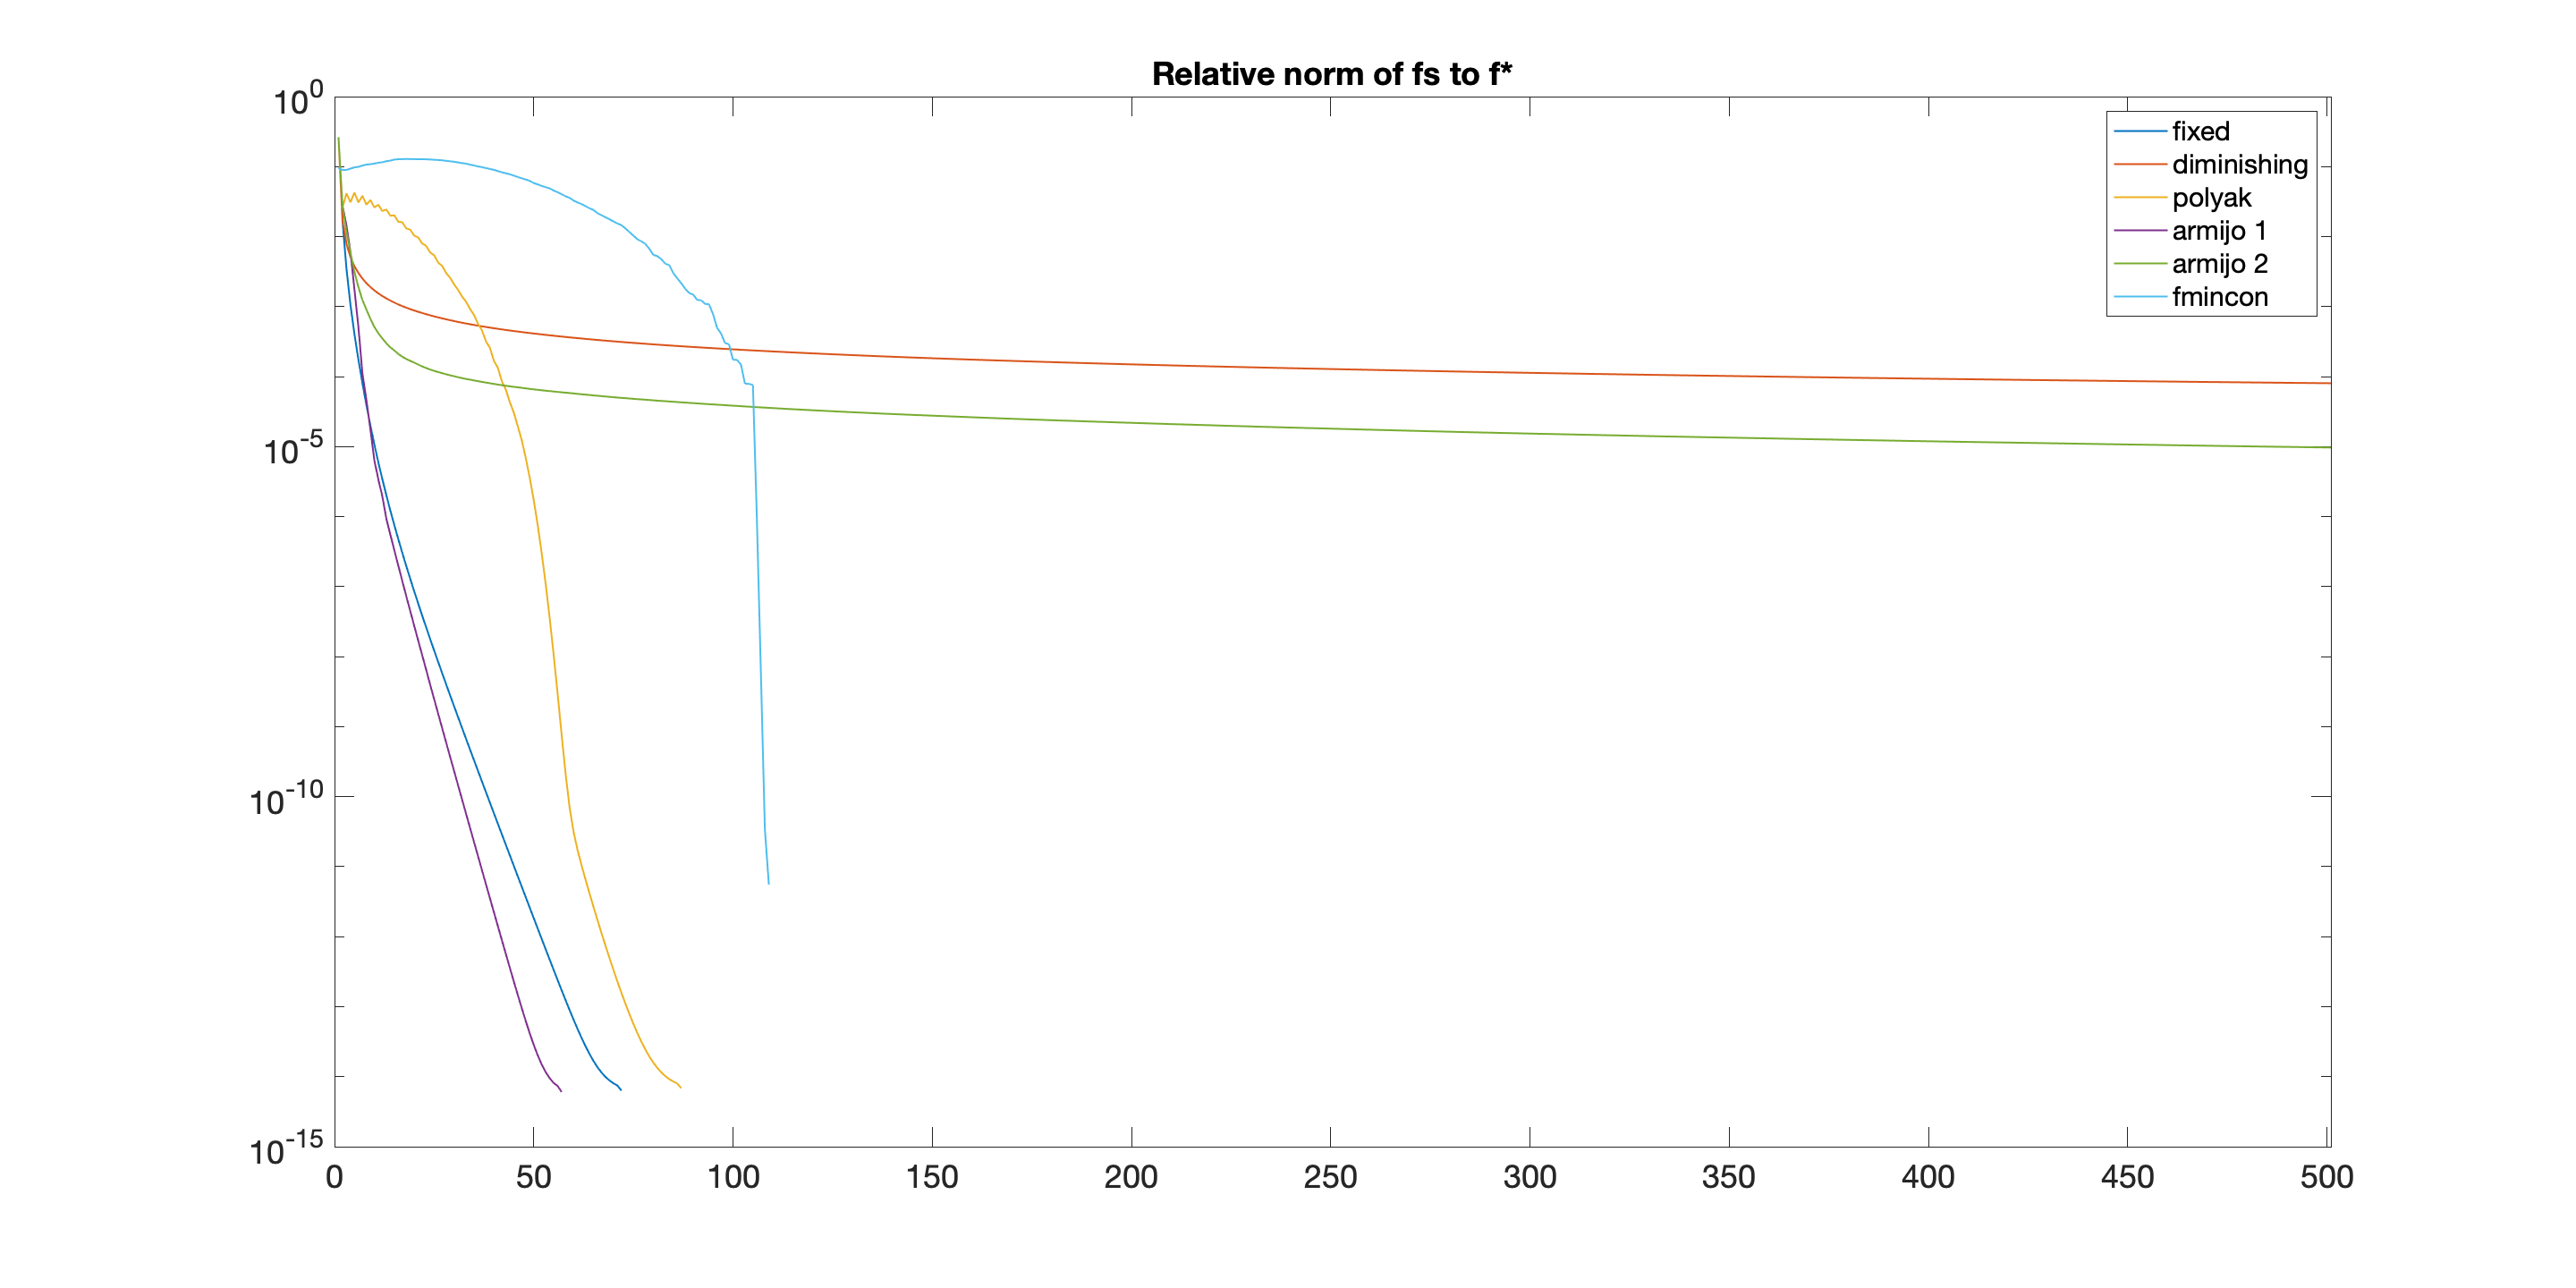
\includegraphics[width=20cm, center]{./plots/plot_100_menouno_zerodue.png}
    \caption{Convergence plot for n = 100, intersection\_percentage = 0.2, actv\_percentage = -1}
    \label{fig:100_menouno_zerodue}
\end{figure} 




% n = 100, actv_percentage = 0.2, intersection_percentage = 0.2

\begin{table}[H]
\setlength{\tabcolsep}{10pt} % Default value: 6pt
\renewcommand{\arraystretch}{1.2} % Default value: 1
\centering
\begin{tabular}{|ccccc|}
\hline
\multicolumn{1}{|c||}{metodo}   & \multicolumn{1}{c|}{mean timing (s)}    & \multicolumn{1}{c|}{std timing (s)} & \multicolumn{1}{c|}{mean of $\frac{\|f - f^*\|}{\|f^*\|}$}   & std of $\frac{\|f - f^*\|}{\|f^*\|}$ \\ \hline\hline
\multicolumn{1}{|c||}{fmincon} & \multicolumn{1}{c|}{2.007301e-01} & \multicolumn{1}{c|}{4.491358e-02}  & \multicolumn{1}{c|}{1.541725e-10} & 5.270178e-19 \\ \hline\hline
\multicolumn{1}{|c||}{fixed}       & \multicolumn{1}{c|}{1.222169e-02} & \multicolumn{1}{c|}{3.575494e-03}  & \multicolumn{1}{c|}{3.937487e-14} & 3.138226e-27  \\ \hline
\multicolumn{1}{|c||}{diminishing} & \multicolumn{1}{c|}{1.113613e-01} & \multicolumn{1}{c|}{1.446869e-02}  & \multicolumn{1}{c|}{1.332589e-03} & 4.294719e-06 \\ \hline
\multicolumn{1}{|c||}{polyak} & \multicolumn{1}{c|}{2.188802e-02} & \multicolumn{1}{c|}{8.299930e-03}  & \multicolumn{1}{c|}{3.218906e-14} & 5.023156e-27 \\ \hline
\multicolumn{1}{|c||}{armijo$_i$} & \multicolumn{1}{c|}{9.888070e-02} & \multicolumn{1}{c|}{3.206025e-02}  & \multicolumn{1}{c|}{3.394667e-14} & 6.875397e-27 \\ \hline
\multicolumn{1}{|c||}{armijo$_{ii}$} & \multicolumn{1}{c|}{2.335504e-01} & \multicolumn{1}{c|}{3.487865e-02}  & \multicolumn{1}{c|}{2.050850e-04} & 1.712115e-07 \\ \hline
\end{tabular}
\caption{Results for n = 100, intersection\_percentage = 0.2, actv\_percentage = 0.2}
\label{tab:100_zerodue_zerodue}
\end{table}


\begin{figure}[H]
\centering
    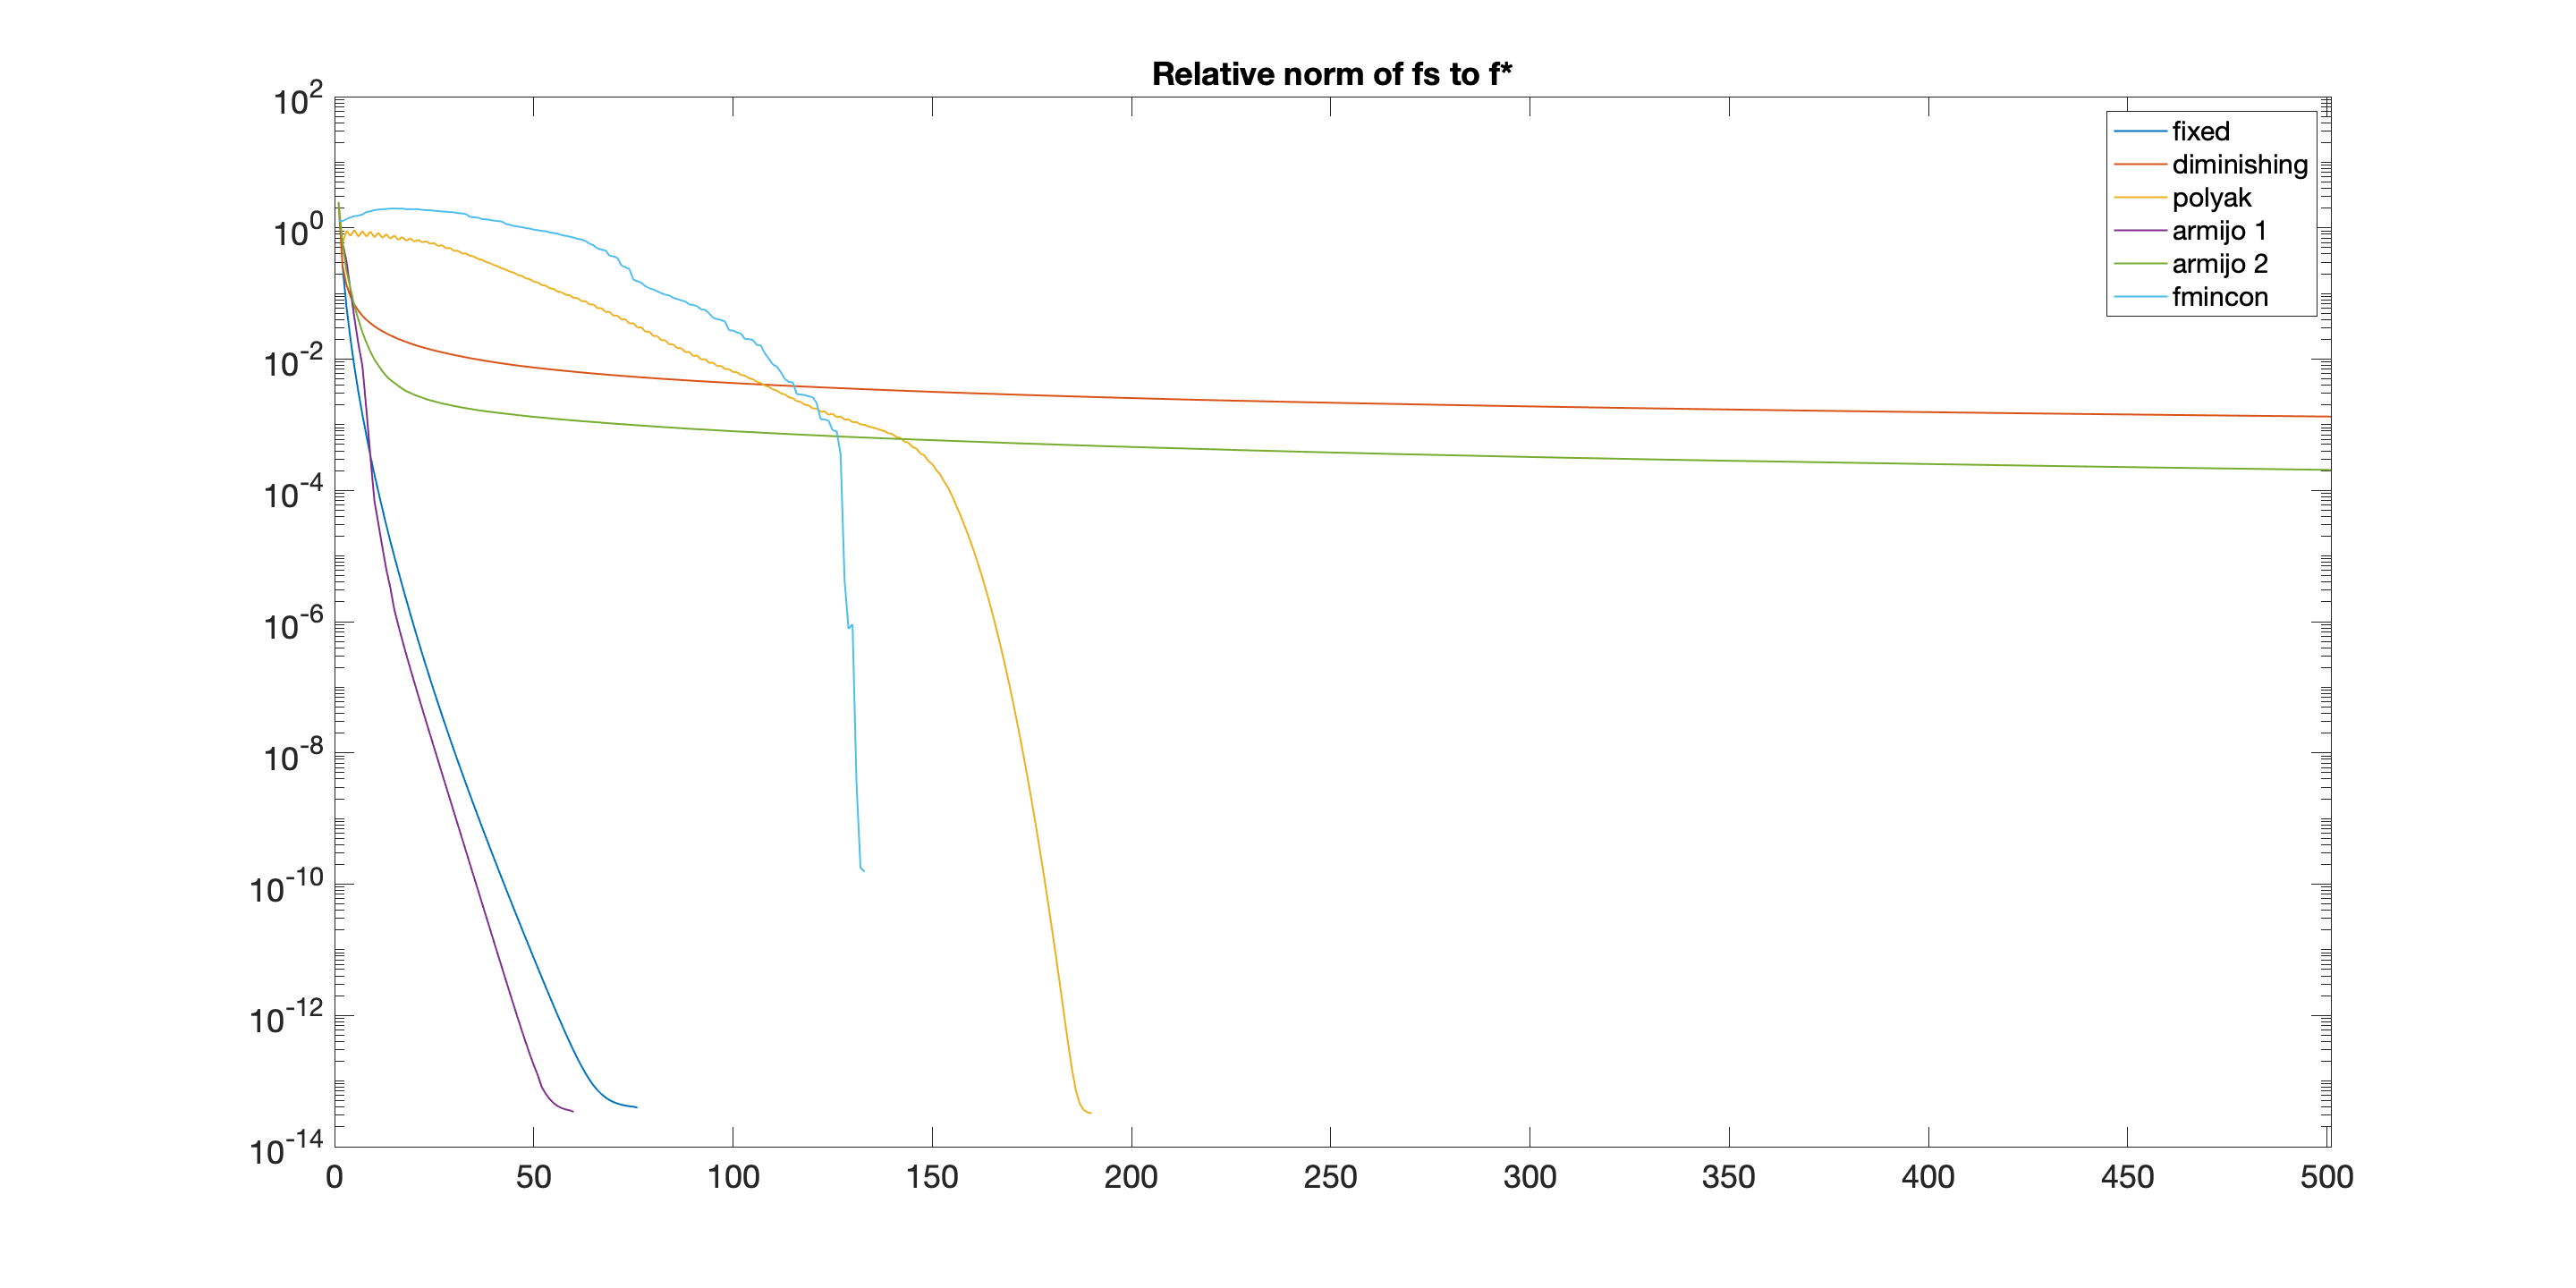
\includegraphics[width=20cm, center]{./plots/plot_100_zerodue_zerodue.png}
    \caption{Convergence plot for n = 100, intersection\_percentage = 0.2, actv\_percentage = 0.2}
    \label{fig:100_zerodue_zerodue}
\end{figure} 



% n = 100, actv_percentage = 0.9, intersection_percentage = 0.2

\begin{table}[H]
\setlength{\tabcolsep}{10pt} % Default value: 6pt
\renewcommand{\arraystretch}{1.2} % Default value: 1
\centering
\begin{tabular}{|ccccc|} 
\hline 
\multicolumn{1}{|c||}{metodo}   & \multicolumn{1}{c|}{mean timing (s)}    & \multicolumn{1}{c|}{std timing (s)} & \multicolumn{1}{c|}{mean of $\frac{\|f - f^*\|}{\|f^*\|}$}   & std of $\frac{\|f - f^*\|}{\|f^*\|}$ \\ \hline\hline 
\multicolumn{1}{|c||}{fmincon}       & \multicolumn{1}{c|}{2.280607e-01} & \multicolumn{1}{c|}{5.461533e-02}  & \multicolumn{1}{c|}{4.575104e-08} & 2.020549e-13  \\ \hline \hline
\multicolumn{1}{|c||}{fixed}       & \multicolumn{1}{c|}{1.385670e-02} & \multicolumn{1}{c|}{4.482161e-03}  & \multicolumn{1}{c|}{7.157249e-13} & 3.599319e-23  \\ \hline 
\multicolumn{1}{|c||}{diminishing}       & \multicolumn{1}{c|}{1.198556e-01} & \multicolumn{1}{c|}{1.789878e-02}  & \multicolumn{1}{c|}{6.681678e-02} & 3.482551e-01  \\ \hline 
\multicolumn{1}{|c||}{polyak}       & \multicolumn{1}{c|}{2.545656e-02} & \multicolumn{1}{c|}{1.071652e-02}  & \multicolumn{1}{c|}{4.227248e-13} & 1.225048e-23  \\ \hline 
\multicolumn{1}{|c||}{armijo$_{i}$}       & \multicolumn{1}{c|}{1.150781e-01} & \multicolumn{1}{c|}{4.508705e-02}  & \multicolumn{1}{c|}{3.626585e-13} & 9.005459e-24  \\ \hline 
\multicolumn{1}{|c||}{armijo$_{ii}$}       & \multicolumn{1}{c|}{2.592929e-01} & \multicolumn{1}{c|}{5.724945e-02}  & \multicolumn{1}{c|}{7.205241e-03} & 4.404590e-03  \\ \hline 
\end{tabular} 

\caption{Results for n = 100, intersection\_percentage = 0.2, actv\_percentage = 0.9}
\label{tab:100_zeronove_zerodue}
\end{table}


\begin{figure}[H]
\centering
    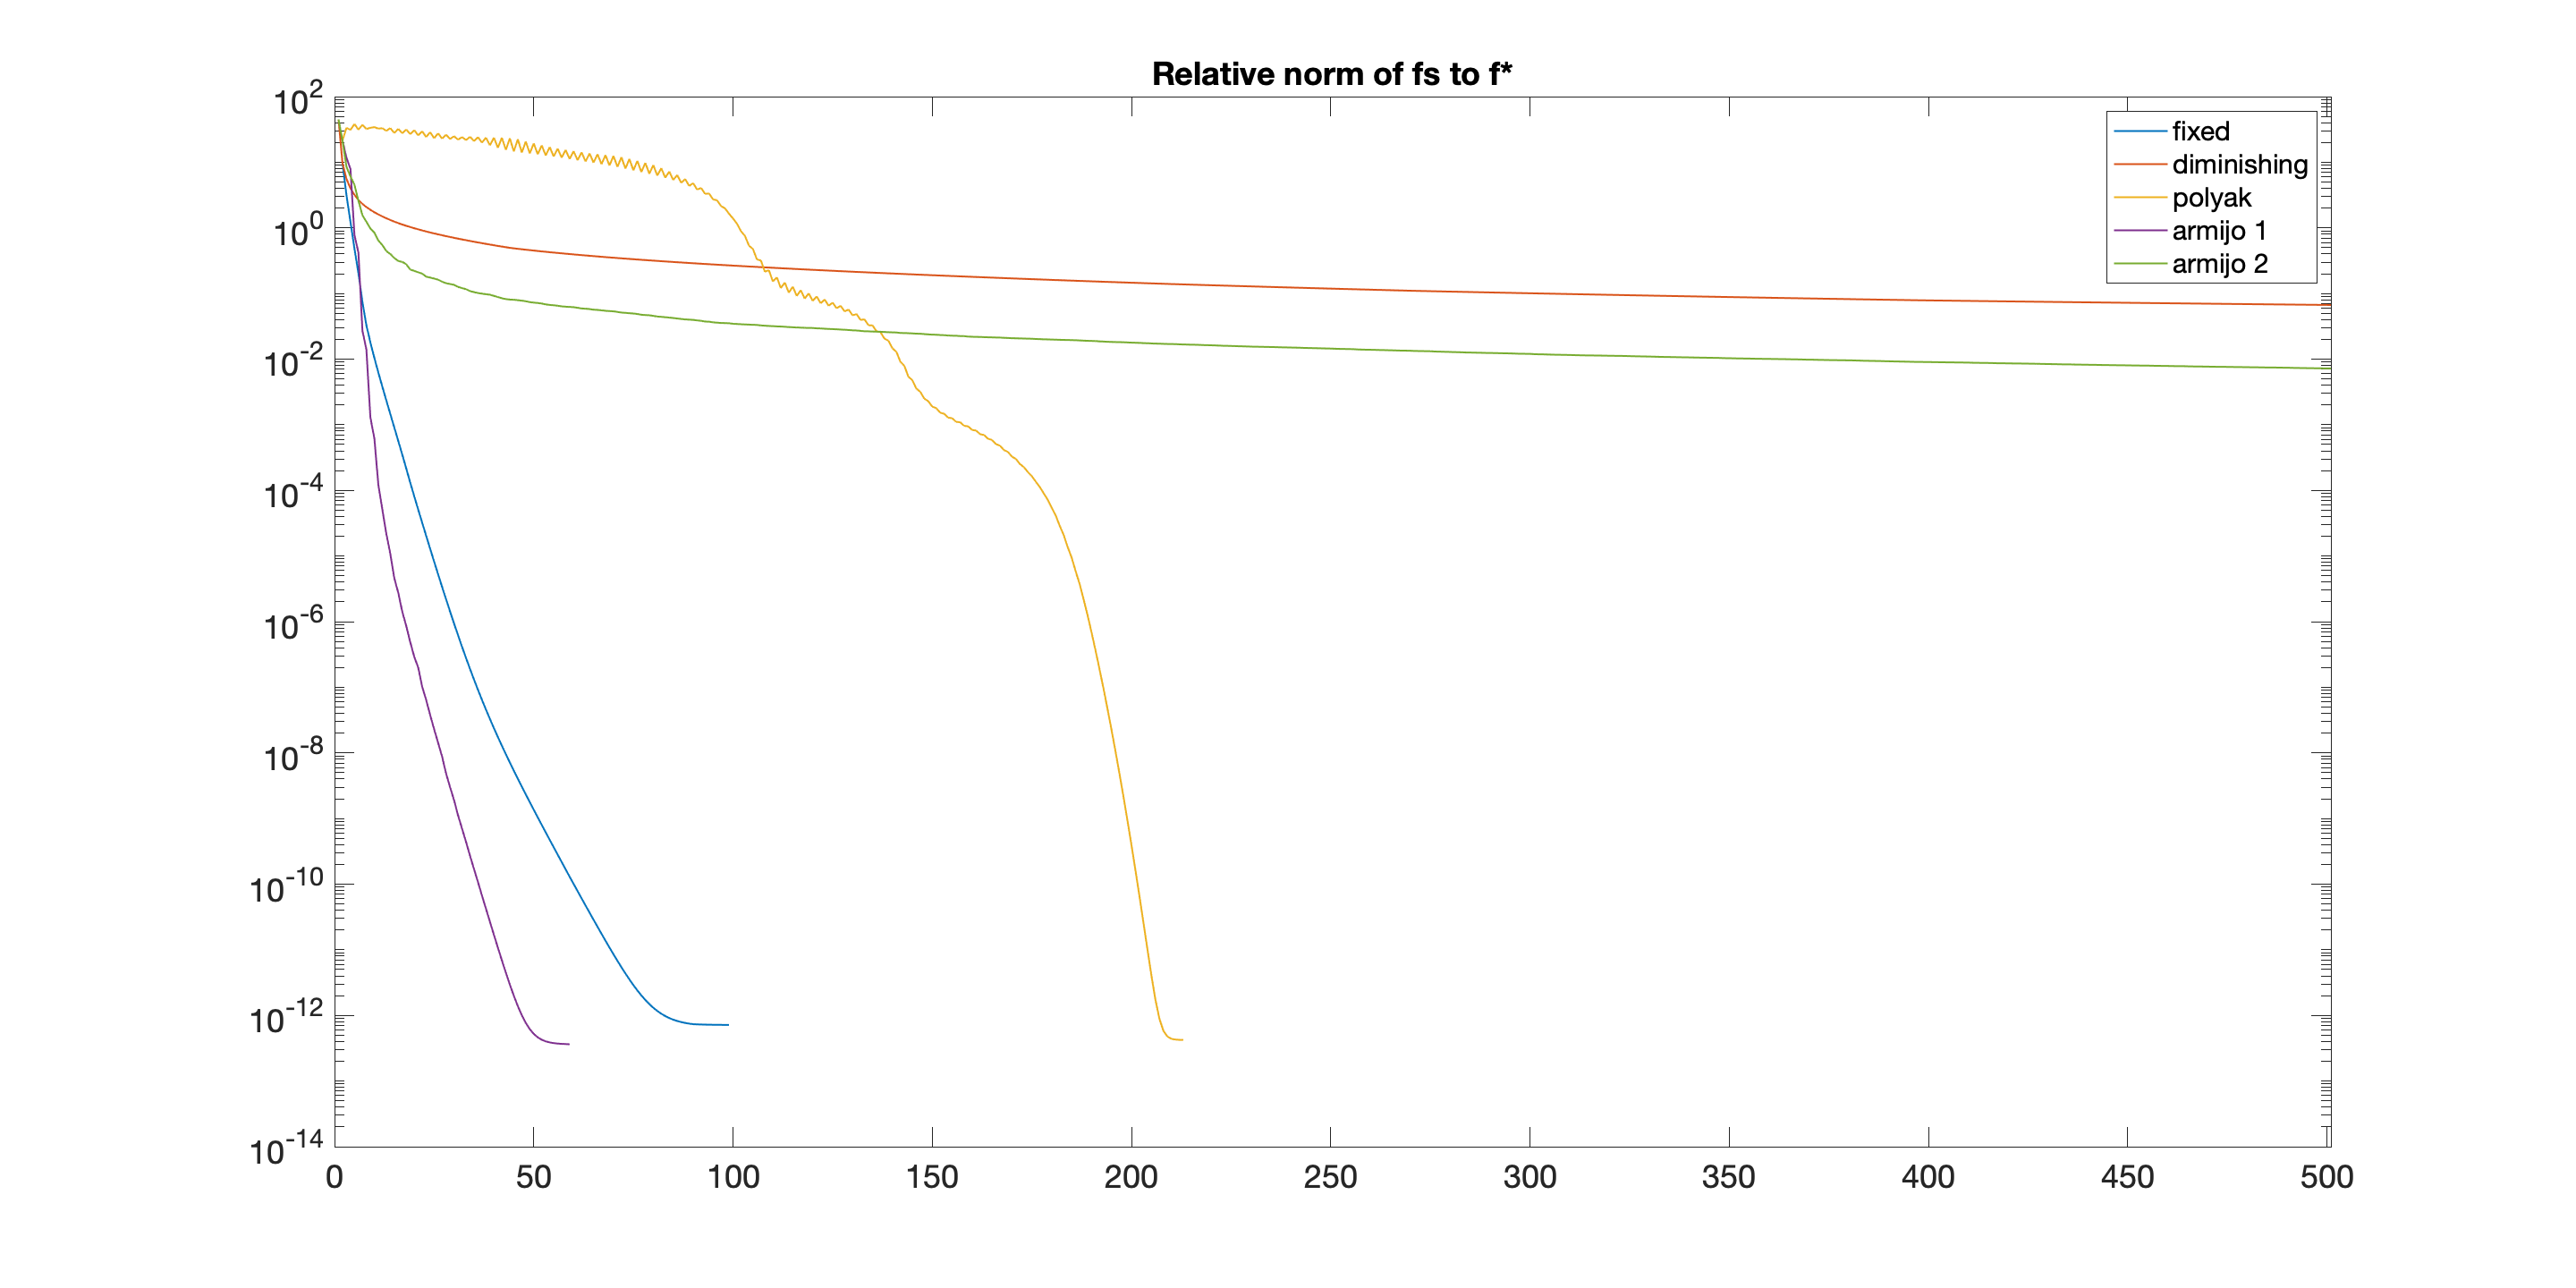
\includegraphics[width=20cm, center]{./plots/plot_100_zeronove_zerodue.png}
    \caption{Convergence plot for n = 100, intersection\_percentage = 0.2, actv\_percentage = 0.9}
    \label{fig:100_zeronove_zerodue}
\end{figure} 



% n = 100, actv_percentage = -1, intersection_percentage = 0.9

\begin{table}[H]
\setlength{\tabcolsep}{10pt} % Default value: 6pt
\renewcommand{\arraystretch}{1.2} % Default value: 1
\centering
\begin{tabular}{|ccccc|} 
\hline 
\multicolumn{1}{|c||}{metodo}   & \multicolumn{1}{c|}{mean timing (s)}    & \multicolumn{1}{c|}{std timing (s)} & \multicolumn{1}{c|}{mean of $\frac{\|f - f^*\|}{\|f^*\|}$}   & std of $\frac{\|f - f^*\|}{\|f^*\|}$ \\ \hline\hline 
\multicolumn{1}{|c||}{fmincon}       & \multicolumn{1}{c|}{2.073557e-01,} & \multicolumn{1}{c|}{4.977241e-02}  & \multicolumn{1}{c|}{2.046668e-11} & 2.319203e-21  \\ \hline \hline
\multicolumn{1}{|c||}{fixed}       & \multicolumn{1}{c|}{1.623224e-02} & \multicolumn{1}{c|}{6.400464e-03}  & \multicolumn{1}{c|}{1.221435e-14} & 6.490718e-28  \\ \hline 
\multicolumn{1}{|c||}{diminishing}       & \multicolumn{1}{c|}{1.269200e-01} & \multicolumn{1}{c|}{2.183725e-02}  & \multicolumn{1}{c|}{4.351213e-04} & 1.845316e-07  \\ \hline 
\multicolumn{1}{|c||}{polyak}       & \multicolumn{1}{c|}{2.026503e-02,} & \multicolumn{1}{c|}{9.366150e-03}  & \multicolumn{1}{c|}{1.276344e-14} & 7.182056e-28  \\ \hline 
\multicolumn{1}{|c||}{armijo$_{i}$}       & \multicolumn{1}{c|}{1.245273e-01,} & \multicolumn{1}{c|}{4.894641e-02}  & \multicolumn{1}{c|}{1.089082e-12} & 1.167740e-22  \\ \hline 
\multicolumn{1}{|c||}{armijo$_{ii}$}       & \multicolumn{1}{c|}{2.597869e-01,} & \multicolumn{1}{c|}{5.744174e-02}  & \multicolumn{1}{c|}{3.441938e-05} & 6.026573e-10  \\ \hline 
\end{tabular} 
\caption{Results for n = 100, intersection\_percentage = 0.9, actv\_percentage = -1}
\label{tab:100_menouno_zeronove}
\end{table}


\begin{figure}[H]
\centering
    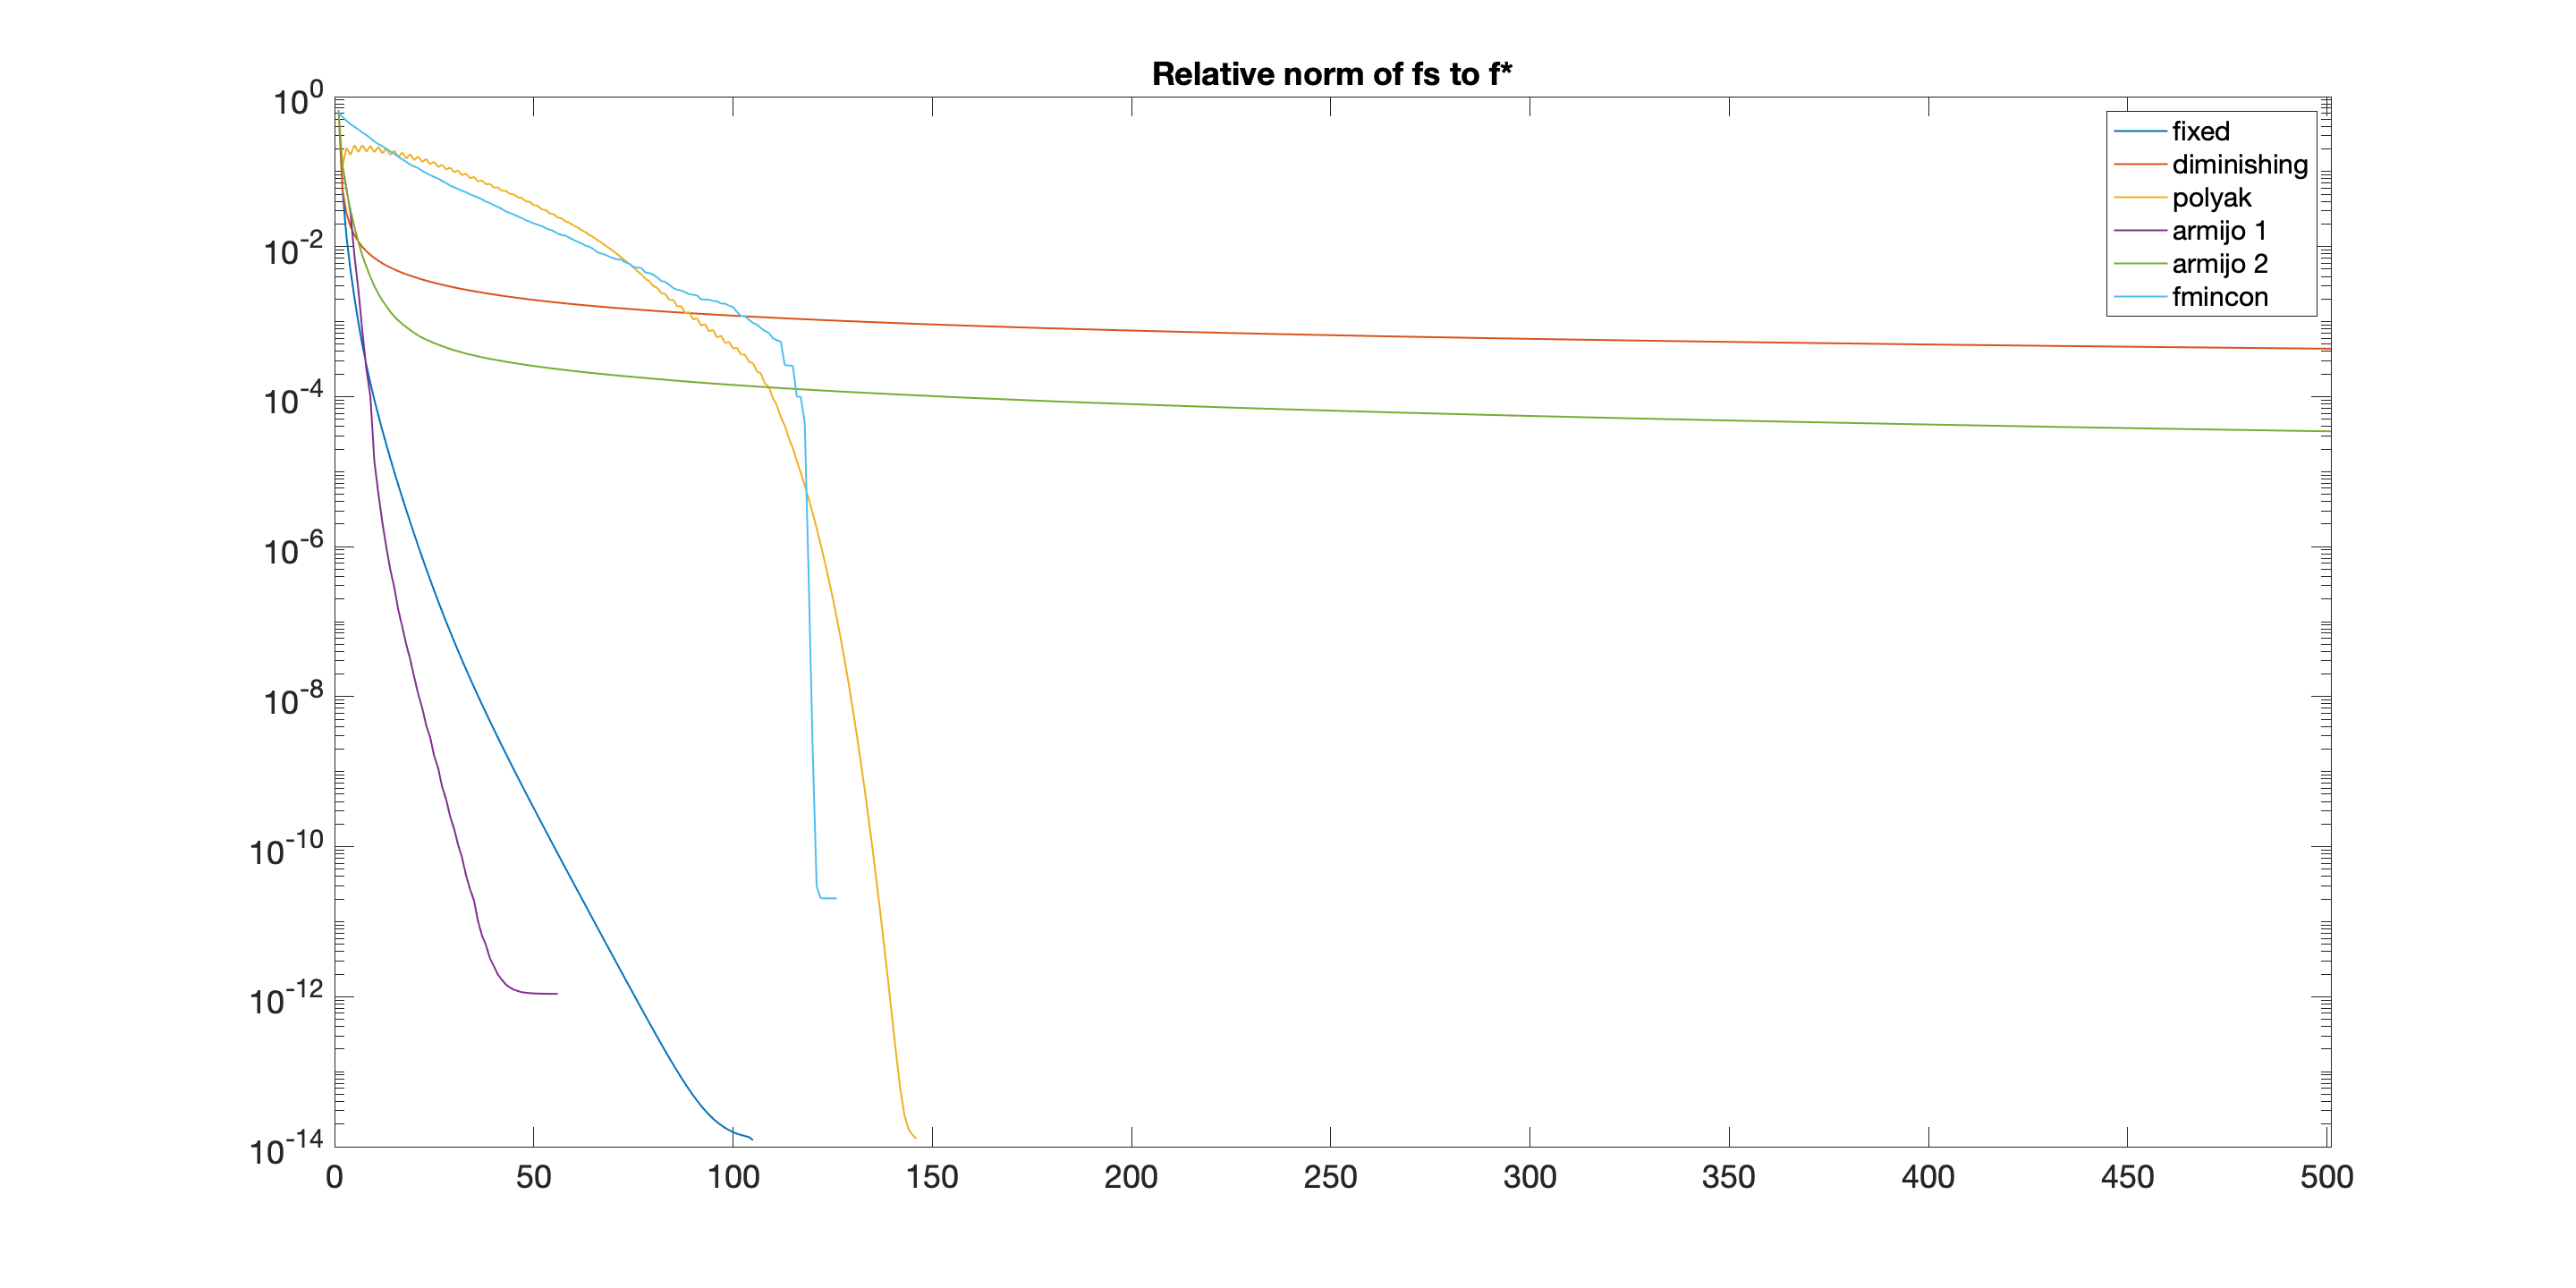
\includegraphics[width=20cm, center]{./plots/plot_100_menouno_zeronove.png}
    \caption{Convergence plot for n = 100, intersection\_percentage = 0.9, actv\_percentage = -1}
    \label{fig:100_menouno_zeronove}
\end{figure} 


% n = 100, actv_percentage = 0.2, intersection_percentage = 0.9

\begin{table}[H]
\setlength{\tabcolsep}{10pt} % Default value: 6pt
\renewcommand{\arraystretch}{1.2} % Default value: 1
\centering
\begin{tabular}{|ccccc|} 
\hline 
\multicolumn{1}{|c||}{metodo}   & \multicolumn{1}{c|}{mean timing (s)}    & \multicolumn{1}{c|}{std timing (s)} & \multicolumn{1}{c|}{mean of $\frac{\|f - f^*\|}{\|f^*\|}$}   & std of $\frac{\|f - f^*\|}{\|f^*\|}$ \\ \hline\hline 
\multicolumn{1}{|c||}{fmincon}       & \multicolumn{1}{c|}{2.177809e-01} & \multicolumn{1}{c|}{3.896319e-02}  & \multicolumn{1}{c|}{9.043926e-10} & 2.349415e-17  \\ \hline \hline
\multicolumn{1}{|c||}{fixed}       & \multicolumn{1}{c|}{1.498239e-02} & \multicolumn{1}{c|}{6.314315e-03}  & \multicolumn{1}{c|}{2.962425e-13} & 1.094444e-24  \\ \hline 
\multicolumn{1}{|c||}{diminishing}       & \multicolumn{1}{c|}{1.224596e-01} & \multicolumn{1}{c|}{2.111157e-02}  & \multicolumn{1}{c|}{2.188161e-02} & 5.449598e-03  \\ \hline 
\multicolumn{1}{|c||}{polyak}       & \multicolumn{1}{c|}{2.878615e-02} & \multicolumn{1}{c|}{1.253583e-02}  & \multicolumn{1}{c|}{7.545432e-14} & 6.020333e-26  \\ \hline 
\multicolumn{1}{|c||}{armijo$_{i}$}       & \multicolumn{1}{c|}{1.166680e-01} & \multicolumn{1}{c|}{4.108040e-02}  & \multicolumn{1}{c|}{5.633356e-14} & 1.934205e-26  \\ \hline 
\multicolumn{1}{|c||}{armijo$_{ii}$}       & \multicolumn{1}{c|}{2.543104e-01} & \multicolumn{1}{c|}{5.127593e-02}  & \multicolumn{1}{c|}{1.519357e-03} & 2.516096e-05  \\ \hline 
\end{tabular} 


\caption{Results for n = 100, intersection\_percentage = 0.9, actv\_percentage = 0.2}
\label{tab:100_zerodue_zeronove}
\end{table}


\begin{figure}[H]
\centering
    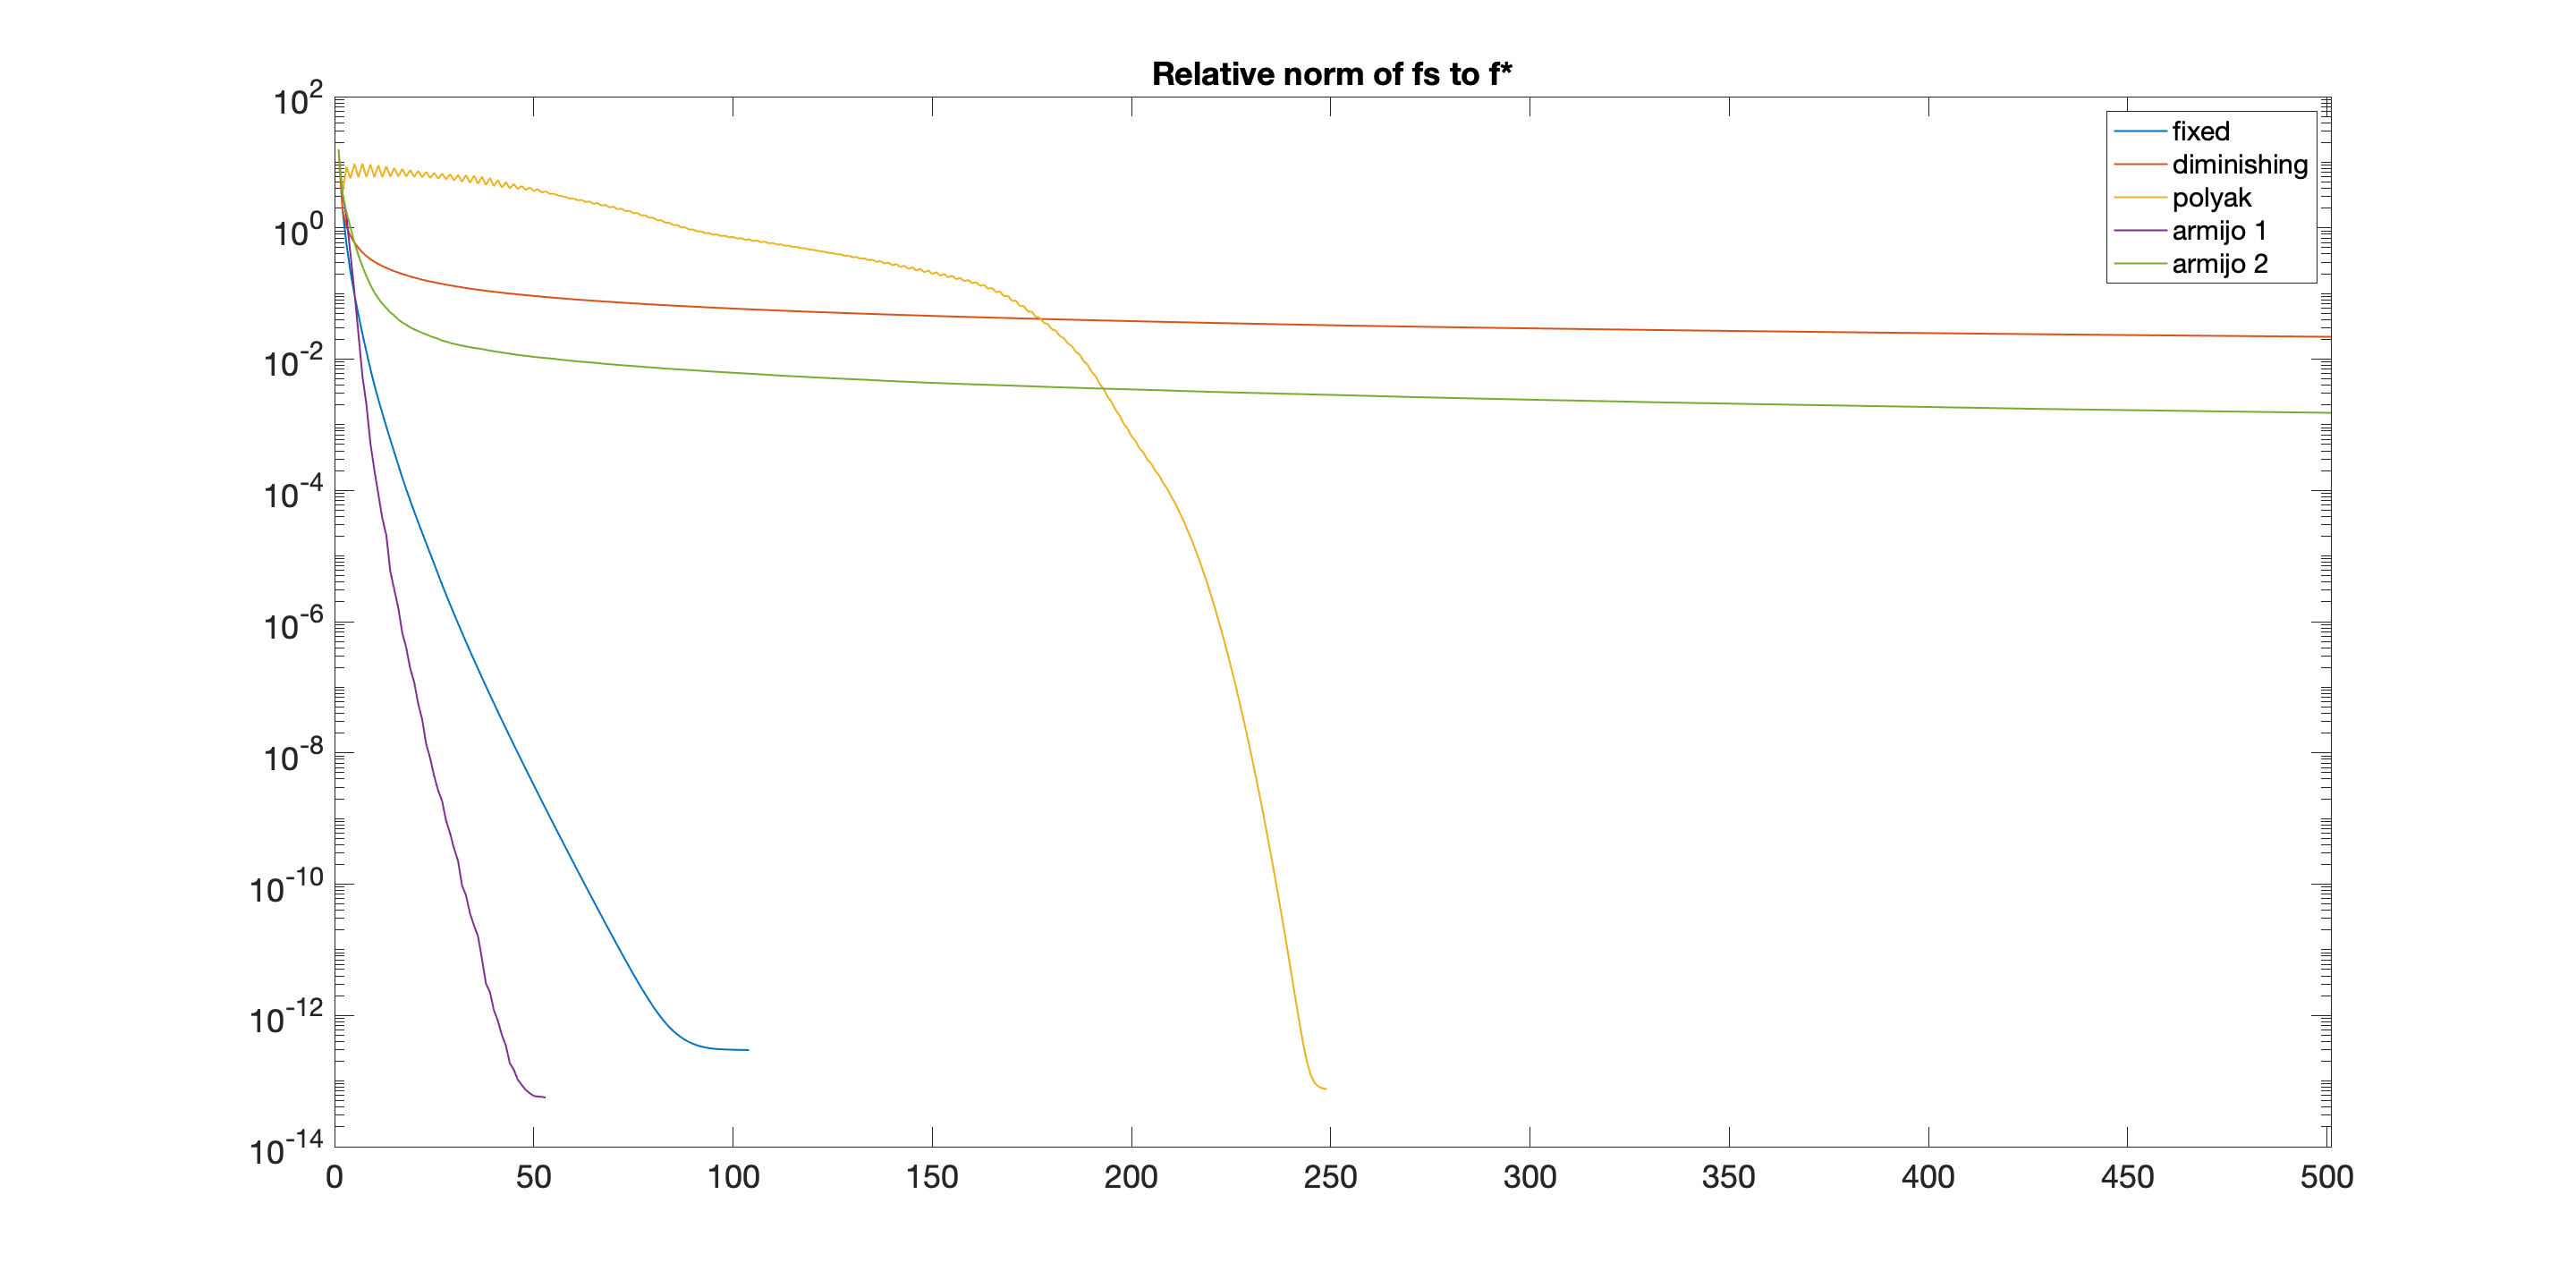
\includegraphics[width=20cm, center]{./plots/plot_100_zerodue_zeronove.png}
    \caption{Convergence plot for n = 100, intersection\_percentage = 0.9, actv\_percentage = 0.2}
    \label{fig:100_zerodue_zeronove}
\end{figure} 



% n = 100, actv_percentage = 0.9, intersection_percentage = 0.9

\begin{table}[H]
\setlength{\tabcolsep}{10pt} % Default value: 6pt
\renewcommand{\arraystretch}{1.2} % Default value: 1
\centering
\begin{tabular}{|ccccc|} 
\hline 
\multicolumn{1}{|c||}{metodo}   & \multicolumn{1}{c|}{mean timing (s)}    & \multicolumn{1}{c|}{std timing (s)} & \multicolumn{1}{c|}{mean of $\frac{\|f - f^*\|}{\|f^*\|}$}   & std of $\frac{\|f - f^*\|}{\|f^*\|}$ \\ \hline\hline 
\multicolumn{1}{|c||}{fmincon}       & \multicolumn{1}{c|}{2.702551e-01} & \multicolumn{1}{c|}{6.115383e-02}  & \multicolumn{1}{c|}{5.822033e-11} & 2.162201e-20  \\ \hline \hline
\multicolumn{1}{|c||}{fixed}       & \multicolumn{1}{c|}{2.454957e-02} & \multicolumn{1}{c|}{9.668051e-03}  & \multicolumn{1}{c|}{1.362308e-13} & 3.186431e-25  \\ \hline 
\multicolumn{1}{|c||}{diminishing}       & \multicolumn{1}{c|}{1.155775e-01} & \multicolumn{1}{c|}{2.330400e-02}  & \multicolumn{1}{c|}{1.134532e-02} & 2.259791e-03  \\ \hline 
\multicolumn{1}{|c||}{polyak}       & \multicolumn{1}{c|}{7.883645e-02} & \multicolumn{1}{c|}{4.082236e-02}  & \multicolumn{1}{c|}{2.285445e-02} & 2.142805e-03  \\ \hline 
\multicolumn{1}{|c||}{armijo$_{i}$}       & \multicolumn{1}{c|}{2.343289e-01} & \multicolumn{1}{c|}{1.116169e-01}  & \multicolumn{1}{c|}{4.404544e-14} & 3.556356e-26  \\ \hline 
\multicolumn{1}{|c||}{armijo$_{ii}$}       & \multicolumn{1}{c|}{2.507455e-01} & \multicolumn{1}{c|}{4.162506e-02}  & \multicolumn{1}{c|}{7.962401e-04} & 1.879149e-05  \\ \hline 
\end{tabular} 

\caption{Results for n = 100, intersection\_percentage = 0.9, actv\_percentage = 0.9}
\label{tab:100_zeronove_zeronove}
\end{table}


\begin{figure}[H]
\centering
    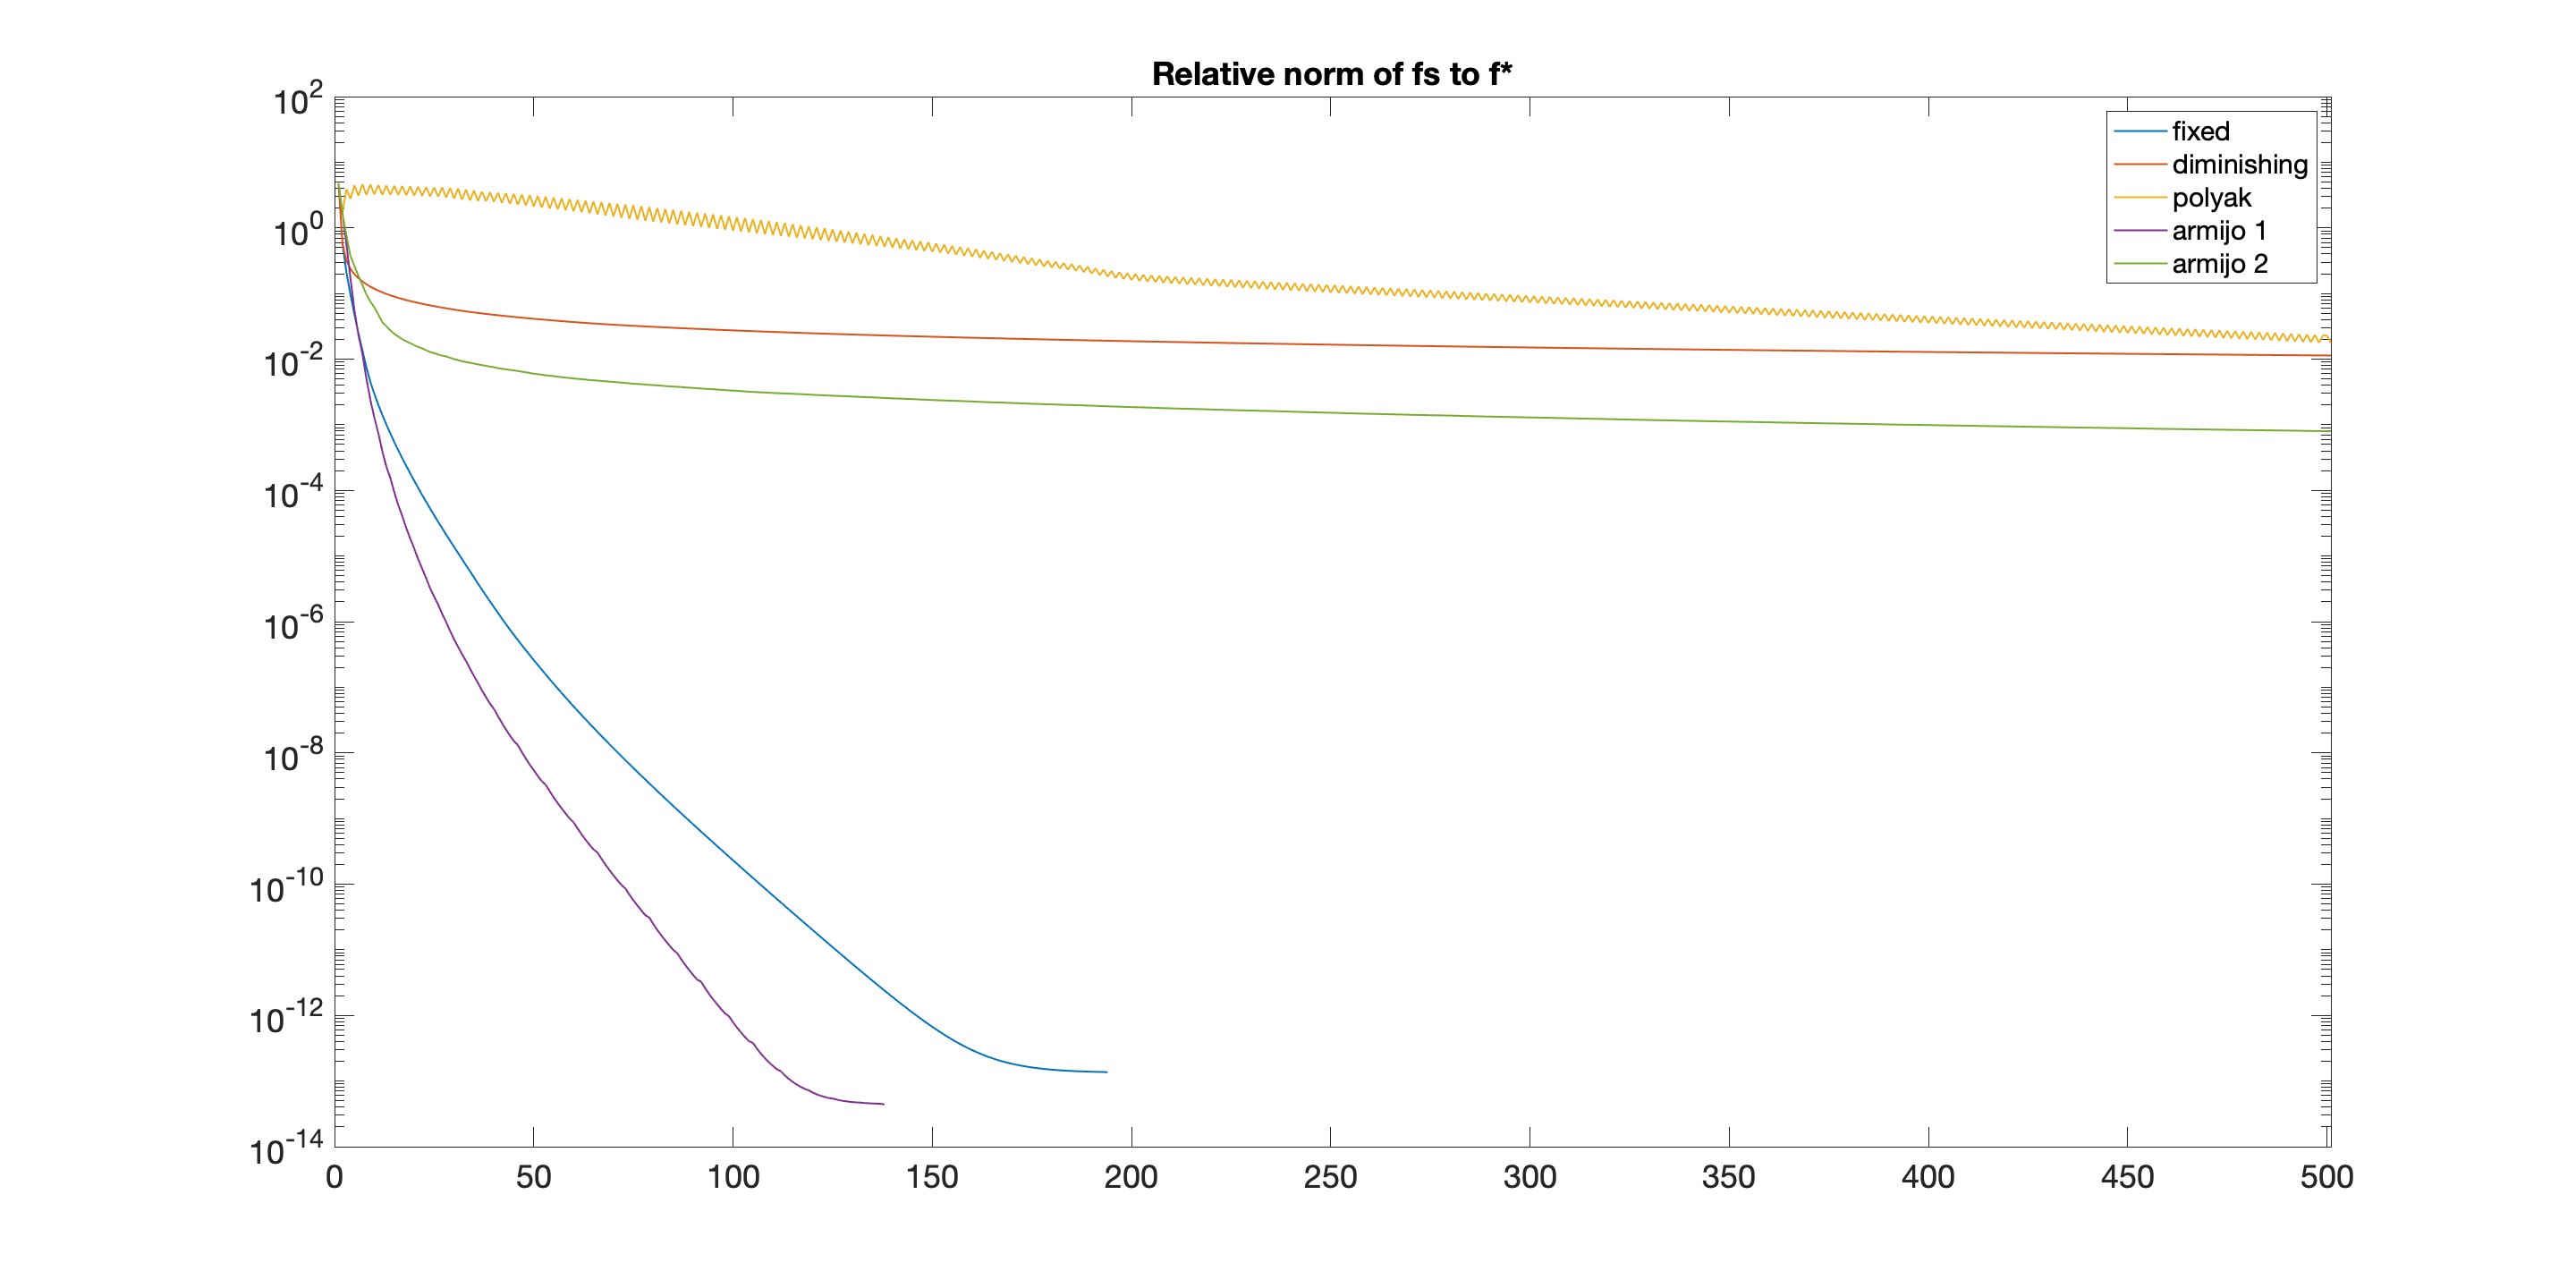
\includegraphics[width=20cm, center]{./plots/plot_100_zeronove_zeronove.png}
    \caption{Convergence plot for n = 100, intersection\_percentage = 0.9, actv\_percentage = 0.9}
    \label{fig:100_zeronove_zeronove}
\end{figure} 



% n = 300

\begin{table}[H]
\setlength{\tabcolsep}{10pt} % Default value: 6pt
\renewcommand{\arraystretch}{1.2} % Default value: 1
\centering
\begin{tabular}{|ccccc|} 
\hline 
\multicolumn{1}{|c||}{metodo}   & \multicolumn{1}{c|}{mean timing (s)}    & \multicolumn{1}{c|}{std timing (s)} & \multicolumn{1}{c|}{mean of $\frac{\|f - f^*\|}{\|f^*\|}$}   & std of $\frac{\|f - f^*\|}{\|f^*\|}$ \\ \hline\hline 
\multicolumn{1}{|c||}{fmincon}       & \multicolumn{1}{c|}{2.590368e+00} & \multicolumn{1}{c|}{5.277532e-01}  & \multicolumn{1}{c|}{5.600965e-12} & 1.633105e-22  \\ \hline \hline
\multicolumn{1}{|c||}{fixed}       & \multicolumn{1}{c|}{3.930736e-02} & \multicolumn{1}{c|}{1.231947e-02}  & \multicolumn{1}{c|}{4.204993e-15} & 7.185436e-29  \\ \hline 
\multicolumn{1}{|c||}{diminishing}       & \multicolumn{1}{c|}{2.972718e-01} & \multicolumn{1}{c|}{6.914928e-02}  & \multicolumn{1}{c|}{4.782880e-04} & 1.325816e-07  \\ \hline 
\multicolumn{1}{|c||}{polyak}       & \multicolumn{1}{c|}{5.253568e-02} & \multicolumn{1}{c|}{1.985033e-02}  & \multicolumn{1}{c|}{4.172296e-15} & 7.501491e-29  \\ \hline 
\multicolumn{1}{|c||}{armijo$_{i}$}       & \multicolumn{1}{c|}{4.587901e-01} & \multicolumn{1}{c|}{1.650006e-01}  & \multicolumn{1}{c|}{3.066231e-15} & 9.026005e-29  \\ \hline 
\multicolumn{1}{|c||}{armijo$_{ii}$}       & \multicolumn{1}{c|}{8.042102e-01} & \multicolumn{1}{c|}{9.428493e-02}  & \multicolumn{1}{c|}{3.454432e-05} & 3.264398e-10  \\ \hline 
\end{tabular}

\caption{Results for n = 300}
\label{tab:300}
\end{table}


\begin{figure}[H]
\centering
    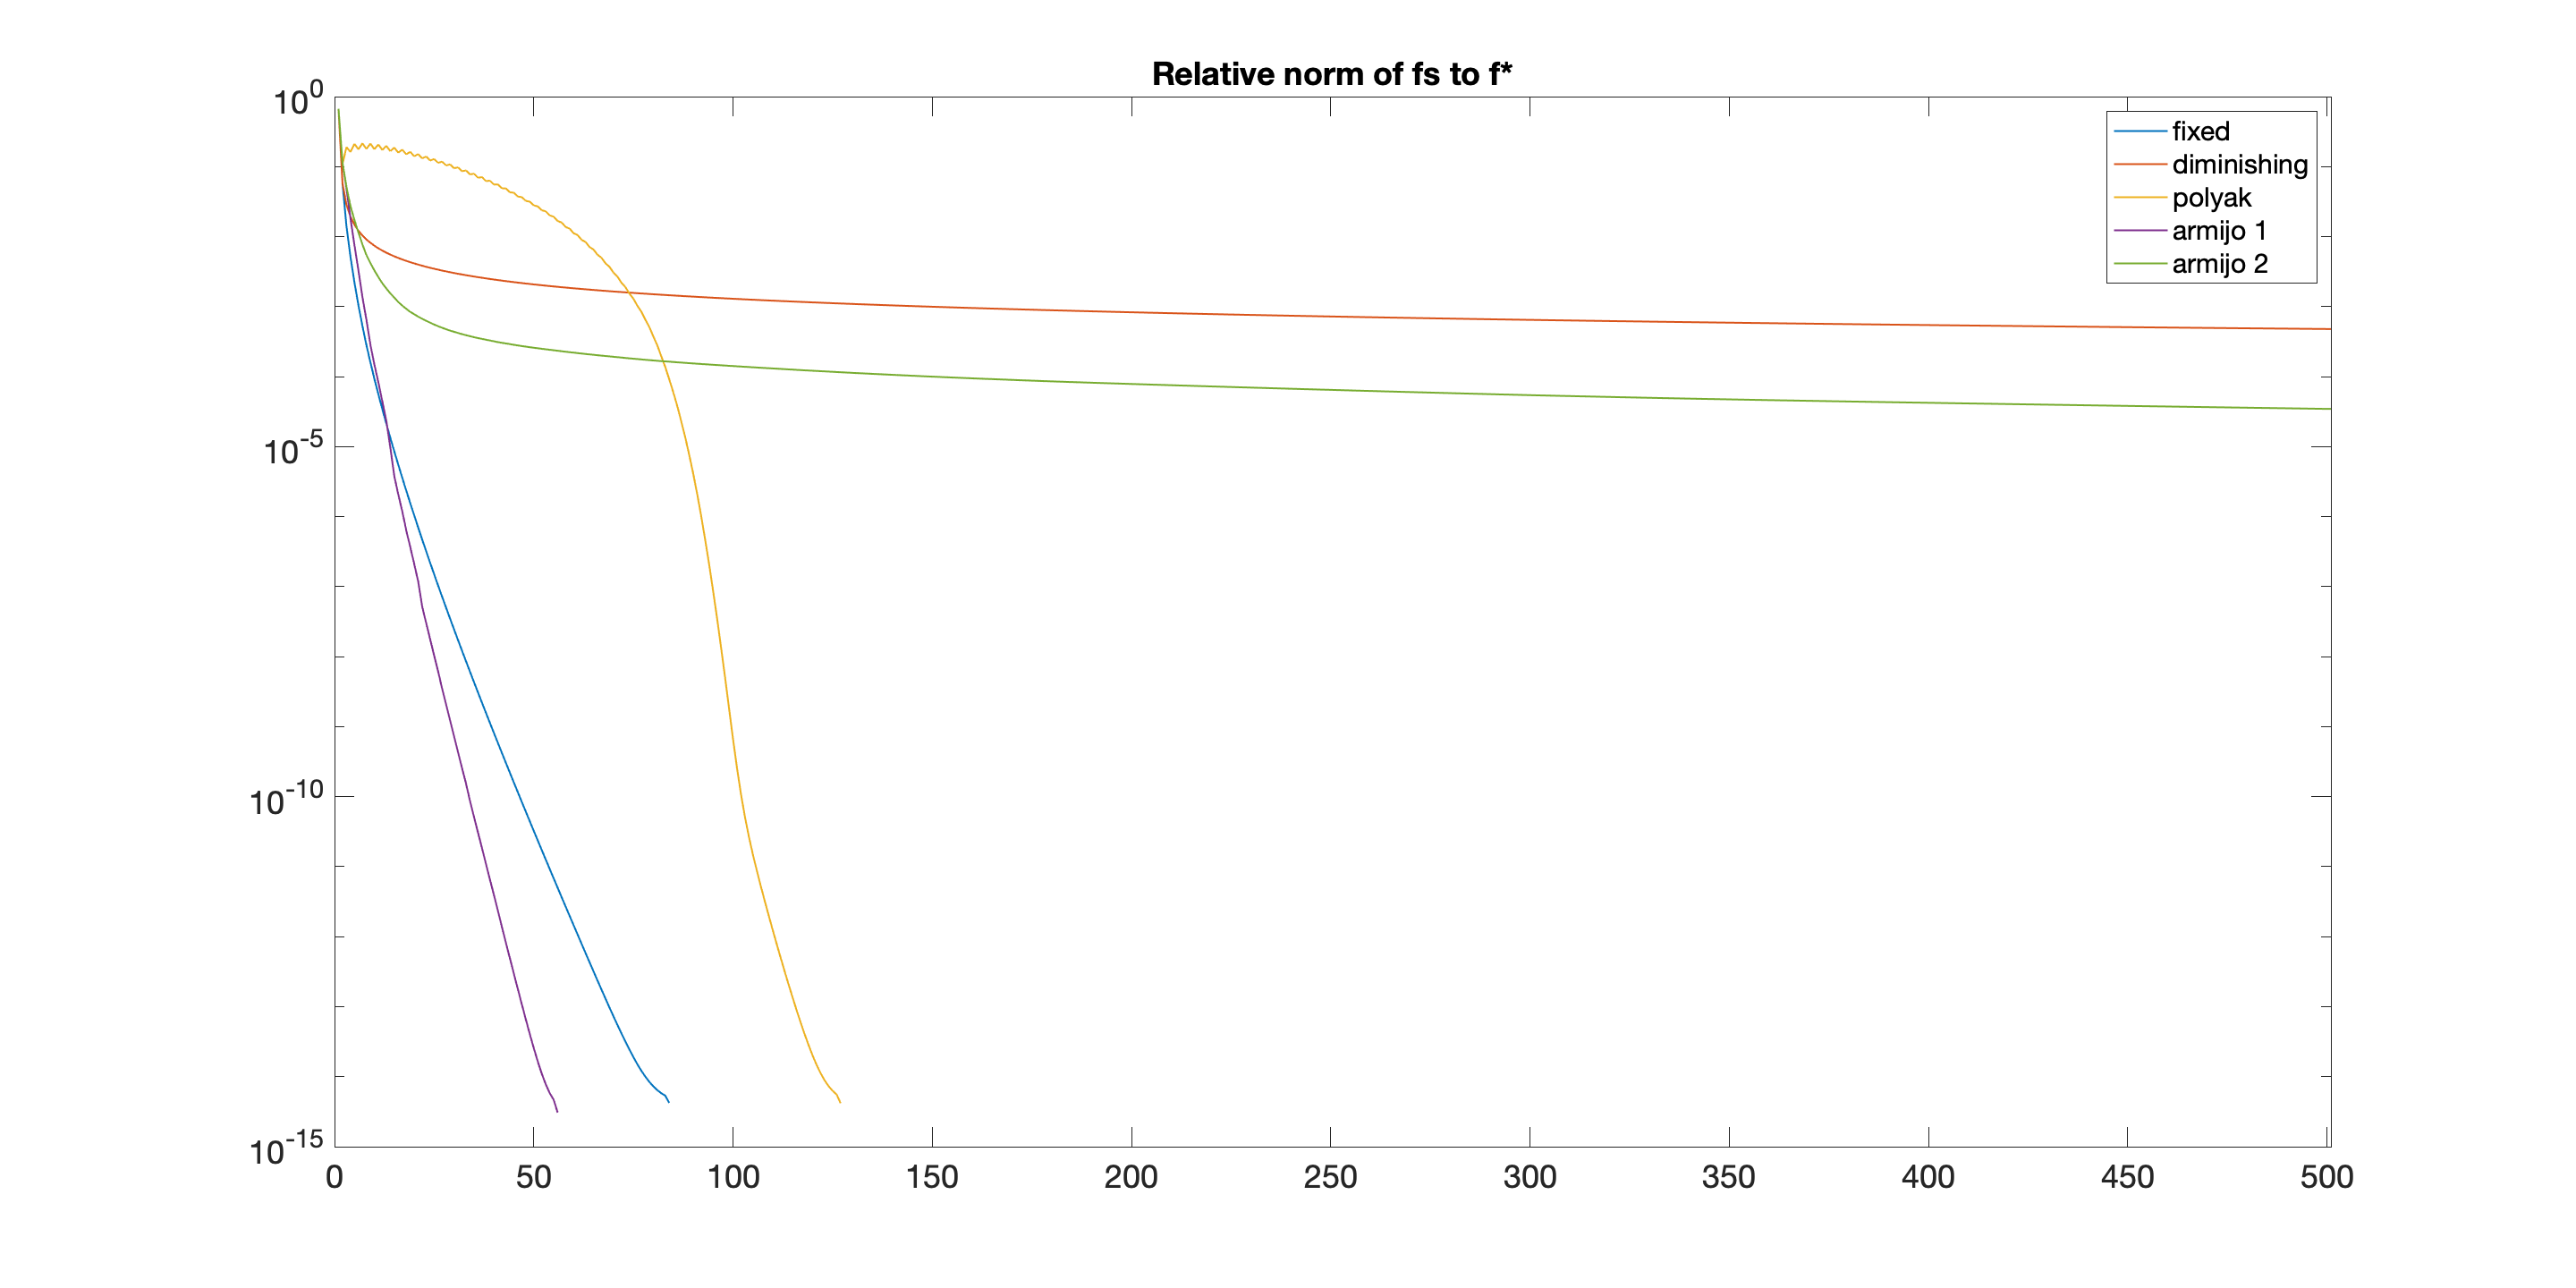
\includegraphics[width=20cm, center]{./plots/plot_300.png}
    \caption{Convergence plot for n = 300}
    \label{fig:300}
\end{figure} 
\section{Support Vector Machine}
Una versione leggermente diversa del problema di ottimizzazione quadratica esposto nella presente trattazione, è alla base del funzionamento delle macchine a vettori di supporto (SVM), ovvero dei modelli di machine learning sfruttati per classificazione e regressione.\\
In questa sezione tratteremo la soft-margin svm lineare per la classificazione, tali modelli di apprendimento possono essere ampliati per la gestione di dati non linearmente separabili, tramite i kernel tricks.
Non tratteremo l'utilizzo di tali modelli per la regressione, sono comunque ben noti metodologie per effettuare regressione, i quali si basano sugli stessi principi matematici sfruttati per effettuare classificazione.\\
I risultati esposti e le notazioni, presenti nella sottosezione di formalizzazione del problema, sono stati ripresi in parte dalle slides del corso di \textbf{Machine Learning}.
\subsection{Formalizzazione del problema}
Dato un insieme di dati $T = \{(x_i, d_i)\}_{i=1}^N$ L'obiettivo delle macchine a vettori di supporto con hard-margin è quello di trovare l'iperpiano separatore, definito da $w$ e $b$, tale che:
\[d_i(w'x_i + b) \geq 1 \quad \forall i = 1, ..., N\]
Di tutti gli iperpiani che soddisfano tali disequazioni, vogliamo quelli che hanno $\| w \|$ più piccola possibile, ciò ci garantisce avere il margine di separazione più ampio possibile, essendo la larghezza del margine inversamente proporzionale alla norma di $w$. Un margine ampio implica una capacità di generalizzazione migliore del modello.\\
Un vettore di supporto $x^{(s)}$ è tale se $d^{(s)}(w'x^{(s)} +b) = 1$.\\
Ci rendiamo conto dunque che trovare $w$ in questo modo equivale a risolvere un problema di ottimizzazione convessa, essendo la funzione norma euclidea una funzione convessa. Essendo inoltre un problema con vincoli lineari, differenziabili quindi con una regione ammissibile convessa, valgono le condizioni KKT ed il teorema di dualità forte, per cui è possibile definirne e risolvere il duale, la cui forma risulta essere più conveniente avendo dimensionalità indipendente dalla dimensionalità del problema di partenza e  per l'utilizzo dei kernel tricks (altrimenti non applicabili). La forma del problema duale è la seguente.
\begin{equation}
\begin{aligned}
\max_{\alpha} \quad & \sum_i \alpha_i - \frac{1}{2}\sum_i \sum_j \alpha_i \alpha_j d_i d_j x_i'x_j\\
\textrm{s.t.} \quad & \sum_i \alpha_i d_i = 0\\
  & \alpha_i \geq 0 \quad \forall i = 1, ..., N\\
\end{aligned}
\end{equation}
Per ora abbiamo definito e formalizzato la linear svm hard-margin, la quale assume avere un dataset linearmente separabile senza outlier, assumiamo ora ammettere la presenza di punti che possono essere non perfettamente classificati dal margine separatore, definiamo dunque i modelli svm soft-margin.\\
Introduciamo le slack variables $\xi_i \geq 0$, tali che,
\[d_i(w'x_i + b) \geq 1 - \xi_i \quad \forall i = 1, ..., N\]
I vettori di supporto saranno quei vettori tali che vale l'uguaglianza.\\
Il problema primale, con l'aggiunta delle slack variables, è dunque:\\
\begin{equation}
\begin{aligned}
\min_{w, b, \xi_i} \quad & \frac{1}{2} w'w + C \sum_i \xi_i\\
\textrm{s.t.} \quad & d_i(w'x_i + b) \geq 1 - \xi_i \quad \forall i = 1, ..., N\\
  & \xi_i \geq 0 \quad \forall i = 1, ..., N\\
\end{aligned}
\end{equation}
Notiamo che anche in questo caso abbiamo una funzione obiettivo convessa cosi come la regione ammissibile, possiamo dunque passare al duale e risolvere tale problema.\\
Costruiamo dapprima la lagrangiana del primale.
\[ L = \frac{1}{2}w'w + C \sum_i \xi_i - \sum_i \alpha_i(d_i(w'x_i + b) - 1 + \xi_i) - \sum_i \mu_i \xi_i\]
Dove gli $\alpha_i$ e i $\mu_i$ sono i moltiplicatori di lagrange relativi ai vincoli del primale. A tal punto vogliamo minimizzare la lagrangiana rispetto a $w$, $b$ e $\xi_i$ e massimizzarla rispetto ad $\alpha_i \geq 0$ e $\mu_i \geq 0$, procediamo dunque ponendo le derivate parziali uguali a 0, rispetto a $w$, $b$ e $\xi_i$, essendo le relative funzioni convesse.
\[\frac{\partial L}{\partial w} = w - \sum_i \alpha_i d_i x_i = 0\]
\[\frac{\partial L}{\partial b} = \sum_i \alpha_i d_i = 0\]
\[\frac{\partial L}{\partial \xi_i} = C - \alpha_i - \mu_i = 0\]
Porre uguale a 0 la derivata rispetto a $\xi_i$ ci porta ad avere $C - \mu_i - \alpha_i = 0$ e essendo dunque $\mu_i \geq 0$ abbiamo che $0 \leq \alpha_i \leq C$.\\
Sostituiamo ora $w_o = \sum_i \alpha_i d_i x_i$ nella lagrangiana.\\
\[\frac{1}{2}(\sum_i \alpha_i d_i x_i)'(\sum_j \alpha_j d_j x_j) - \sum_i \sum_j \alpha_i \alpha_j d_i d_j x_i'x_j + \sum_i \alpha_i - \sum_i \alpha_i d_i b - \sum_i (C - \mu_i - \alpha_i) \xi_i\]
Applicando le uguaglianze date dalle derivate abbiamo che la funzione lagrangiana minimizzata rispetto ad $w$, $b$ e $\xi_i$ è data dalla seguente.
\[\sum_i \alpha_i - \frac{1}{2}\sum_i \sum_j \alpha_i \alpha_j d_i d_j x_i'x_j\]
A tal punto è diretta la formulazione del duale, mettendo insieme le equazioni dettate fin'ora.\\
\begin{equation}
\begin{aligned}
\max_{\alpha} \quad & \sum_i \alpha_i - \frac{1}{2}\sum_i \sum_j \alpha_i \alpha_j d_i d_j x_i'x_j\\
\textrm{s.t.} \quad & \sum_i \alpha_i d_i = 0\\
  & 0 \leq \alpha_i \leq C \quad \forall i = 1, ..., N\\
\end{aligned}
\end{equation}
\'E diretto notare che tale problema di ottimizzazione quadratica è affine al problema presentato nella prima parte della presente trattazione, l'unica differenza è quella di avere l'uguaglianza al posto della disuguaglianza nel vincolo di zaino.
\'E comunque possibile applicare il metodo risolutivo del gradiente proiettato per trovare l'ottimo del duale, trovando un punto di minimo dell'opposto della funzione obiettivo e facendo una leggera modifica alla funzione di proiezione.
\subsection{Esperimenti}
Per fini didattici abbiamo implementato la soft-margin svm in matlab sfruttando il metodo risolutivo tramite gradiente proiettato per programmazione quadratica con vincoli di knapsack, abbiamo dunque, utilizzato le diverse scelte del passo fissando il numero massimo di iterazioni a 1000, confrontato tali metodi con il modello implementato dalla \texttt{fitcsvm} di matlab, disponibile tramite \texttt{statistics and machine learning toolbox}.
Il dataset su cui abbiamo effettuato tali esperimenti è \texttt{Ionosphere} disponibile built-in in matlab. Tale dataset consiste in una matrice \texttt{X} di dimensioni 351(samples) x 34(features), contenente valori reali i quali rappresentano informazioni riguardanti la ionosfera. La variabile target è definita da un vettore \texttt{Y} contenente i valori 'g' e 'b', che indicano la qualità dei segnali radar. Per maggiorni informazioni si faccia riferimento a \cite{ionosphere_dataset}.\\
Non si sono effettuate fasi di preprocessing dei dati di input, l'unica operazione sui dati effettuata è stata quella di trasformare il vettore \texttt{Y} sostituendo i valori \quotes{g} con 1 e \quotes{b} in -1.\\
Abbiamo suddiviso il dataset in una parte di training per l'allenamento dei modelli $80\%$, e la restante parte per il testing, prima di effettuare tale divisione il dataset è sottoposto ad operazione di shuffling.\\
Si è dunque effettuata una fase di screening per la selezione (a grandi linee) dei parametri algoritmici, dalla quale si è selezionato il valore $C=10$.\\
Nella tabella \ref{table:svmresults} si riportano, per ogni metodo, il tempo allenamento, il valore di accuracy nel dataset di training e testing, il valore di precision e recall per il dataset di testing.\\
Notiamo come i valori di accuracy, precision e recall, sono abbastanza simili tra i vari metodi, mentre i valori di timing sono più elevati per le due varianti del metodo di Armijo, ciò è sicuramente dovuto alla ricerca di backtracking.\\
\begin{table}[H]
    \setlength{\tabcolsep}{10pt} % Default value: 6pt
    \renewcommand{\arraystretch}{1.2} % Default value: 1
    \centering
    \begin{tabular}{ |p{3cm}||p{1.5cm}|p{2cm}|p{2cm}|p{2cm}|p{1.5cm}|  }
    \hline
    metodo & timing (s) & accuracy tr \% & accuracy ts \% & precision ts \% & recall ts \%\\
    \hline
    \hline
    fitcsvm (MATLAB) & 0.69  & 95 & 83 & 78 & 72\\
    \hline
    \hline
    Fixed ($\alpha = 0.001$) & 0.69 & 90 & 86 & 86 & 72\\
    \hline
    Diminishing ($\alpha_k = \frac{1}{k}$) & 0.64 & 94 & 76 & 67 & 64\\
    \hline
    Polyak ($\delta_k = \frac{1}{k}$) & 0.55 & 90 & 85 & 85 & 68\\
    \hline
    Armijo ($\beta = 0.5 \quad \sigma = 0.1$) & 5.24 & 91 & 80 & 72 & 72\\
    \hline
    Armijo 2 ($\beta = 0.5 \quad \sigma = 0.1$) & 1.79 & 90 & 82 & 80 & 64\\
    \hline
    \end{tabular}
    \caption{Risultati SVM, Ionosphere dataset}
    \label{table:svmresults}
\end{table}
\bibliographystyle{plain}
\bibliography{bibliography.bib}
\end{document}

